% Chương Hệ hỗ trợ ra quyết định
% Số liệu lấy từ results/cum6 và results/cum6b. Bảng d_*.tex do python/tao_bang_tex_dss.py sinh, hình d_chon_k.png và d_man_hinh_*.png do python/ve_hinh_dss.py sinh.
% Hình d_do_nhay.png và d_mo_phong.png do python/ve_hinh_mohinh.py sinh. Không sửa tay số liệu trong latex/bang/.
% Mỗi mục đi theo một câu hỏi của người quản lý, thiết kế và kết quả chạy thật viết chung.
\section{Thiết kế và hiện thực hệ hỗ trợ ra quyết định}

Chương 5 cho ra xác suất không mua lại của từng khách. Chương này biến xác suất đó thành quyết định. Người quản lý cần trả lời bốn câu hỏi: chọn khách nào trong ngân sách (mục 6.2), khách thuộc nhóm nào (6.3), chăm sóc bằng cách nào (6.4) và đặt ngân sách bao nhiêu khi chưa biết chăm sóc có hiệu quả không (6.5). Mục 6.1 nêu bài toán và kiến trúc, mục 6.6 trình bày giao diện và bản demo. Trừ khi nói khác, số liệu tính tại mốc chấm điểm 08/07/2014 cho 18.360 khách.

\subsection{Bài toán và kiến trúc DSS}
\subsubsection{Quyết định cần hỗ trợ}
Tại mỗi mốc chấm điểm, với một ngân sách có hạn, người quản lý phải chọn khách nào cần chăm sóc trong 90 ngày tiếp theo và chăm sóc bằng hành động nào. Phải chọn vì không thể chăm sóc tất cả: ngân sách có hạn và 81,2\% khách có nhãn không mua lại (Bảng~\ref{tab:thamso}). Đây là quyết định bán cấu trúc ở cấp quản lý~\cite{turban2011}. Phần có cấu trúc (tính xác suất, giá trị kỳ vọng, chọn khách trong ngân sách) do máy làm. Phần không có cấu trúc (chọn hình thức chăm sóc, cân nhắc thông tin ngoài dữ liệu, chốt ngân sách) do người quản lý làm. Ba nhóm người dùng là quản lý Marketing/Sales (đặt ngân sách, chạy kịch bản, duyệt danh sách), nhân viên phân tích dữ liệu (chấm điểm, theo dõi mô hình, đề xuất quy tắc) và nhân viên chăm sóc khách hàng (thực hiện theo danh sách).

Hai nguyên tắc thiết kế xuyên suốt. Thứ nhất, DSS đề xuất, người dùng quyết định cuối, và người dùng xem được theo rủi ro, theo giá trị hay theo nhóm tuỳ ý~\cite{turban2011}. Thứ hai, xác suất không mua lại chỉ cho biết khách có nguy cơ, không cho biết chăm sóc có làm khách quay lại hay không~\cite{lemmens2020}, nên hiệu quả chăm sóc là tham số do người quản lý giả định và được thử ở mục 6.5.

\subsubsection{Bốn thành phần và bốn pha ra quyết định}
CompanyX DSS gồm bốn thành phần đúng như Chương 2~\cite{tlmh,turban2011} (Bảng~\ref{tab:thanhphan}), mở rộng từ khung dữ liệu, mô hình và giao diện của Sprague~\cite{sprague1980}. Bảng~\ref{tab:quytrinh} ánh xạ bốn pha của Simon~\cite{simon1977,turban2011} (Hình~\ref{fig:simon}) vào câu hỏi của người quản lý và chức năng tương ứng của DSS. Việc gửi chiến dịch nằm ngoài hệ thống, DSS chỉ cung cấp danh sách và khuyến nghị.

\begin{table}[!htbp]
\centering
\caption{Bốn thành phần của CompanyX DSS}
\label{tab:thanhphan}
\footnotesize
\begin{tabular}{p{2.8cm}p{11.6cm}}
\toprule
Thành phần & Nội dung \\
\midrule
Quản lý dữ liệu & Đọc kho \texttt{CompanyX\_DW}, chủ yếu các bảng \texttt{analytics.\allowbreak CustomerSnapshot}, \texttt{analytics.\allowbreak CustomerRiskScore}, và ghi kết quả vào \texttt{CustomerSegment}, \texttt{CareRecommendation} \\
Quản lý mô hình & Naive Bayes (Chương 5), K-means, mô hình giá trị ròng kỳ vọng và bài toán chọn khách trong ngân sách \\
Quản lý tri thức & Kho quy tắc chăm sóc R1 đến R9 (bảng \texttt{analytics.\allowbreak CareRule}) và luật kết hợp gợi ý sản phẩm \\
Giao diện người dùng & Ứng dụng web Streamlit~\cite{streamlit}, cho đổi giả định mà không cần huấn luyện lại mô hình \\
\bottomrule
\end{tabular}
\end{table}

\begin{table}[!htbp]
\centering
\caption{Bốn pha ra quyết định và chức năng DSS hỗ trợ}
\label{tab:quytrinh}
\footnotesize
\begin{tabular}{p{1.9cm}p{3.9cm}p{5.8cm}p{2.2cm}}
\toprule
Pha & Câu hỏi của người quản lý & Chức năng DSS & Mục \\
\midrule
Tìm hiểu & Tình hình khách không mua lại ra sao, nhóm nào đáng lo? & Dashboard tổng quan: tỷ lệ nguy cơ, phân bố xác suất, hạng giá trị, nhóm khách & 6.3 \\
Thiết kế & Có những phương án nào, mỗi phương án cho kết quả ra sao? & Mô hình giá trị kỳ vọng, what-if, độ nhạy & 6.2, 6.5 \\
Lựa chọn & Chọn khách nào, bao nhiêu khách? & Tối ưu trong ngân sách, tìm mục tiêu, danh sách ưu tiên & 6.2, 6.4 \\
Thực hiện & Làm gì với từng khách, kết quả ra sao? & Khuyến nghị theo quy tắc, xuất danh sách, theo dõi mô hình & 6.4, 6.6 \\
\bottomrule
\end{tabular}
\end{table}

\subsection{Chọn khách nào trong ngân sách}
\subsubsection{Giá trị kỳ vọng của việc chăm sóc một khách}
Mô hình xét một lát cắt tại mốc chấm điểm và một chu kỳ 90 ngày sau mốc. Việc khách $i$ có mua lại hay không ($Y_i$) là điều kiện rủi ro: chưa biết trước nhưng có xác suất $p_i$ từ Chương 5. Tỷ lệ chăm sóc thành công $r$ và chi phí $c$ là điều kiện bất định vì chưa có chiến dịch nào để đo, nên người quản lý nhập theo giả định. Bảng~\ref{tab:bien} liệt kê các biến theo ba loại ở Chương 2, thêm biến trung gian, Hình~\ref{fig:influence} vẽ quan hệ giữa chúng: hình chữ nhật là biến quyết định, hình tròn là biến không kiểm soát được hoặc trung gian, hình bầu dục là biến kết quả, mũi tên gấp khúc là quan hệ rủi ro hoặc bất định.

\begin{table}[!htbp]
\centering
\caption{Các biến của mô hình quyết định chăm sóc khách hàng}
\label{tab:bien}
\footnotesize
\begin{tabular}{p{2.4cm}p{1.8cm}p{6.2cm}p{3.8cm}}
\toprule
Loại biến & Ký hiệu & Ý nghĩa & Nguồn hoặc giá trị \\
\midrule
Biến quyết định & $x_i$ & Chăm sóc khách $i$ ($x_i=1$) hay không ($x_i=0$) & Lời giải của mô hình, người quản lý duyệt \\
Không kiểm soát được & $B$ & Ngân sách chiến dịch, cố định trong một lần giải & Người quản lý nhập \\
Không kiểm soát được & $Y_i$ & Khách $i$ không có đơn hợp lệ trong 90 ngày sau mốc (giá trị quan sát được sau này là nhãn $y_i$ ở Chương 4) & Chưa biết tại mốc \\
Không kiểm soát được & $p_i$ & Xác suất $Y_i=1$ do mô hình phân lớp dự đoán & \texttt{RiskScore} \\
Không kiểm soát được & $AOV_i$ & Giá trị trung bình một đơn của khách $i$ trước mốc (\texttt{SubTotal}, không gồm thuế và phí vận chuyển) & \texttt{FactSalesOrder} \\
Không kiểm soát được & $g$ & Tỷ lệ lợi nhuận gộp trên doanh thu & Tính từ giá vốn các đơn trước mốc \\
Không kiểm soát được & $r$ & Tỷ lệ chăm sóc thành công: xác suất một khách vốn sẽ không mua lại quay lại mua nhờ được chăm sóc & Giả định, người quản lý nhập \\
Không kiểm soát được & $c$ & Chi phí cho mỗi khách được chọn (liên hệ và ưu đãi) & Giả định, người quản lý nhập \\
Trung gian & $v_i=g\cdot AOV_i$ & Lợi nhuận gộp của một lần mua nếu giữ được khách $i$ & Tính từ $AOV_i$ và $g$ \\
Kết quả & $Z=R-C$ & Giá trị ròng kỳ vọng: lợi nhuận gộp kỳ vọng giữ lại $R$ trừ tổng chi phí $C$ & Tính từ mô hình \\
\bottomrule
\end{tabular}
\end{table}

\begin{figure}[!htbp]
\centering
\begin{tikzpicture}[
  dec/.style={draw, rectangle, minimum width=1.0cm, minimum height=0.7cm, font=\small},
  var/.style={draw, circle, minimum size=1.0cm, inner sep=1pt, font=\small},
  res/.style={draw, ellipse, minimum width=1.5cm, minimum height=0.9cm, font=\small},
  cert/.style={-{Stealth[length=2mm]}},
  risk/.style={-{Stealth[length=2mm]}, decorate, decoration={zigzag, amplitude=0.8pt, segment length=4pt}}]
  \node[var] (g) at (0,3.6) {$g$};
  \node[var] (aov) at (0,2.2) {$AOV_i$};
  \node[var] (p) at (0,0.5) {$p_i$};
  \node[var] (y) at (0,-1.0) {$\tilde{Y}_i$};
  \node[var] (r) at (0,-2.5) {$r$};
  \node[var] (v) at (3.0,3.0) {$v_i$};
  \node[var] (R) at (6.0,0.4) {$R$};
  \node[dec] (x) at (3.0,-3.0) {$x_i$};
  \node[var] (B) at (0,-4.2) {$B$};
  \node[var] (c) at (3.0,-5.2) {$c$};
  \node[var] (C) at (6.0,-3.6) {$C$};
  \node[res] (Z) at (9.2,-1.6) {$Z$};
  \draw[cert] (g) -- (v);
  \draw[cert] (aov) -- (v);
  \draw[cert] (v) -- (R);
  \draw[cert] (p) -- (y);
  \draw[risk] (y) -- (R);
  \draw[risk] (r) -- (R);
  \draw[cert] (x) -- (R);
  \draw[cert] (x) -- (C);
  \draw[cert] (c) -- (C);
  \draw[cert] (B) -- node[above, font=\scriptsize] {ràng buộc} (x);
  \draw[cert] (R) -- (Z);
  \draw[cert] (C) -- (Z);
\end{tikzpicture}

\caption{Sơ đồ ảnh hưởng của mô hình quyết định chăm sóc khách hàng}
\label{fig:influence}
\end{figure}

Với một khách $i$ có hai phương án: chăm sóc hoặc không. Bảng~\ref{tab:payoffhai} tính kết quả của hai phương án theo hai trạng thái của khách, lấy chênh lệch so với không chăm sóc. Bảng dựa trên hai giả định: $r$ chỉ tính trên khách sẽ rời bỏ nếu không được chăm sóc, và chăm sóc không đổi hành vi của khách vốn sẽ quay lại.

\begin{table}[!htbp]
\centering
\caption{Bảng kết quả của hai phương án đối với khách $i$}
\label{tab:payoffhai}
\footnotesize
\begin{tabular}{p{3.0cm}p{4.0cm}p{4.0cm}p{2.8cm}}
\toprule
Phương án & Khách sẽ rời bỏ (xác suất $p_i$) & Khách vẫn quay lại (xác suất $1-p_i$) & Giá trị kỳ vọng \\
\midrule
Không chăm sóc & 0 & 0 & 0 \\
Chăm sóc & $r\, v_i - c$ & $-c$ & $p_i\, r\, v_i - c$ \\
\bottomrule
\end{tabular}
\end{table}

Giá trị kỳ vọng của việc chăm sóc khách $i$ và tiêu chí chọn khách là:
\begin{align}
    v_i &= g \cdot AOV_i, \qquad EV_i = p_i\, r\, v_i - c \label{eq:EV}\\
    \text{chọn chăm sóc khách } i \text{ khi } EV_i > 0 &\iff p_i\, v_i > c/r \quad (r>0) \label{eq:chon}
\end{align}
Ví dụ với $r=10\%$, $c=10$ USD (nên $c/r=100$ USD) và $g=40\%$ (giá trị minh hoạ):
\begin{itemize}
    \item Khách A: $p_i=0{,}90$, $AOV_i=2.500$ USD, $v_i=1.000$ USD, $EV_i=0{,}90 \times 0{,}10 \times 1.000 - 10 = 80$ USD, chọn.
    \item Khách B: $p_i=0{,}98$, $AOV_i=40$ USD, $v_i=16$ USD, $EV_i=0{,}98 \times 0{,}10 \times 16 - 10 = -8{,}43$ USD, không chọn.
    \item Khách C: $p_i=0{,}50$, $AOV_i=2.000$ USD, $v_i=800$ USD, $EV_i=0{,}50 \times 0{,}10 \times 800 - 10 = 30$ USD, chọn.
\end{itemize}
Khách B có xác suất rời bỏ cao nhất nhưng không đáng chăm sóc vì giá trị quá nhỏ. Vì vậy xác suất chỉ là đầu vào, việc chọn khách dựa trên giá trị kỳ vọng. Do $p_i$ nhân thẳng vào $EV_i$, mô hình cần xác suất sát thực tế, đây là lý do Chương 5 theo dõi Brier.

\subsubsection{Bài toán tối ưu và cách giải}
Cộng giá trị kỳ vọng của các khách được chọn ta có $Z$. Bài toán là quy hoạch nguyên 0--1, cùng cấu trúc với bài toán phối hợp sản phẩm ở Chương 2~\cite{turban2011}:
\begin{align}
    \max\; Z &= R - C = \sum_i x_i\, p_i\, r\, v_i - c \sum_i x_i = \sum_i x_i\,(p_i\, r\, v_i - c) \label{eq:muctieu}\\
    \text{với}\quad & c \sum_i x_i \leq B, \qquad x_i \in \{0,1\} \label{eq:rangbuoc}
\end{align}
Chương 5 tính cùng công thức $Z$ với nhãn thật $y_i$ thay cho $p_i$ để so các mô hình. Vì chi phí $c$ như nhau cho mọi khách, lời giải tối ưu là xếp khách theo $p_i v_i$ giảm dần và chọn $K$ khách đầu:
\begin{equation}
    K = \min\left(\lfloor B/c \rfloor,\; n_+\right) \label{eq:K}
\end{equation}
với $\lfloor B/c \rfloor$ là số khách ngân sách cho phép và $n_+$ là số khách có $EV_i>0$. Khi chi phí khác nhau giữa các khách (mục 6.4.3), bài toán thành bài toán cái túi 0--1 và được giải bằng quy hoạch nguyên.

Mô hình có ba giới hạn cần nhớ. $p_i$ học từ lịch sử không có chiến dịch giữ chân nào, nên $Z$ là giá trị kỳ vọng theo giả định, không phải hiệu quả đã đo, muốn đo thật cần chiến dịch có nhóm đối chứng~\cite{lemmens2020}. $v_i$ chỉ tính một lần mua với một tỷ lệ lợi nhuận gộp chung, không phải giá trị vòng đời. $c$ phát sinh cả với khách vốn sẽ quay lại.

\subsubsection{Các đại lượng đo từ dữ liệu}
Bảng~\ref{tab:thamso} là các đại lượng đo được từ kho. Khách không mua lại chiếm 81,2\% (trung bình 19 mốc có nhãn) nên không thể chăm sóc tất cả. 50,5\% khách có $v_i$ nhỏ hơn $c/r = 100$ USD, tức chăm sóc riêng không bù được chi phí. Nếu không tính lợi ích từ khách chưa đến kỳ mua lại, $Z$ cơ sở còn 205.555 USD, nên các giá trị $Z$ dưới đây là cận trên.

\begin{table}[!htbp]
\centering
\caption{Các đại lượng của mô hình giá trị kỳ vọng đo từ dữ liệu}
\label{tab:thamso}
\footnotesize
\begin{tabular}{p{4.6cm}p{3.6cm}p{6.2cm}}
\toprule
Đại lượng & Giá trị & Ghi chú \\
\midrule
Tỷ lệ lợi nhuận gộp g, toàn bộ & 0,4115 & Giá vốn ProductCostHistory tại ngày đặt, 59.795 dòng trong phạm vi \\
g của Bikes / Accessories / Clothing & 0,406 / 0,626 / 0,402 & Bikes chiếm 96,5\% doanh thu \\
Z kịch bản cơ sở nếu dùng g theo nhóm & 290.014 USD (g chung 292.595 USD) & 99,7\% khách trong danh sách giữ nguyên \\
Tỷ lệ khách không mua lại trong 90 ngày ($y=1$) & 81,2\% & Trung bình 19 mốc có nhãn \\
Tỷ trọng Monetary của khách $y=1$ & 78,0\% & Trung bình 19 mốc có nhãn \\
Số đơn trung bình của khách quay lại trong 90 ngày & 1,12 & 93,5\% chỉ đặt một đơn \\
Giá trị đơn khi quay lại so với AOV trước đó (trung vị tỷ số) & 0,87 & Trung bình 1.427 USD so với 1.873 USD \\
Khách có v $<$ c/r = 100 USD tại mốc chấm điểm & 50,5\% & Chăm sóc riêng không bù được chi phí \\
Z cơ sở nếu trừ khách chưa đến kỳ khỏi lợi ích & 205.555 USD (r hoà vốn 1,63\%) & 26,2\% khách $y=1$ theo nhãn 90 ngày tự mua lại trong ngày 90–180 \\
Ngân sách để kênh R4 (nhóm N3) bắt đầu có khách & khoảng 61.213 USD & Dưới mức này lợi trên mỗi USD của khách N3 thấp hơn khách khác \\
\bottomrule
\end{tabular}

\end{table}

\subsubsection{Kết quả kịch bản cơ sở và what-if}
Kịch bản cơ sở là $r=10\%$, $c=10$ USD mỗi khách và $B=40.000$ USD. Với kịch bản này hệ thống chọn 4.000 khách, kỳ vọng giữ lại 358 khách và đạt $Z = 292.595$ USD. Với what-if, người quản lý đổi một tham số rồi xem kết quả (Bảng~\ref{tab:whatif}, Hình~\ref{fig:man3}). Tăng $r$ từ 10\% lên 20\% làm $Z$ tăng lên 625.189 USD, nên tỷ lệ thành công là yếu tố ảnh hưởng lớn nhất. Tăng ngân sách lên 100.000 USD thì DSS chỉ dùng 85.540 USD vì đã hết khách có $EV$ dương. Mỗi lần phân tích, DSS lưu tham số và kết quả thành một kịch bản để so sánh.

\begin{table}[!htbp]
\centering
\caption{Phân tích what-if quanh kịch bản cơ sở}
\label{tab:whatif}
\footnotesize
\resizebox{\textwidth}{!}{\begin{tabular}{lrrrr}
\toprule
Kịch bản & Số khách & Chi phí (USD) & $Z$ (USD) & Chênh so với cơ sở (USD) \\
\midrule
Cơ sở ($r=10\%$, $c=10$ USD, $B=40.000$ USD) & 4.000 & 40.000 & 292.595 & 0 \\
$r=5\%$ & 4.000 & 40.000 & 126.297 & $-$166.297 \\
$r=20\%$ & 4.000 & 40.000 & 625.189 & +332.595 \\
$c=5$ USD & 8.000 & 40.000 & 424.359 & +131.764 \\
$c=20$ USD & 2.000 & 40.000 & 152.066 & $-$140.529 \\
$B=20.000$ USD & 2.000 & 20.000 & 172.066 & $-$120.529 \\
$B=60.000$ USD & 6.000 & 60.000 & 359.388 & +66.793 \\
$B=100.000$ USD & 8.554 & 85.540 & 386.235 & +93.640 \\
\bottomrule
\end{tabular}
}
\end{table}

\begin{figure}[!htbp]
\centering
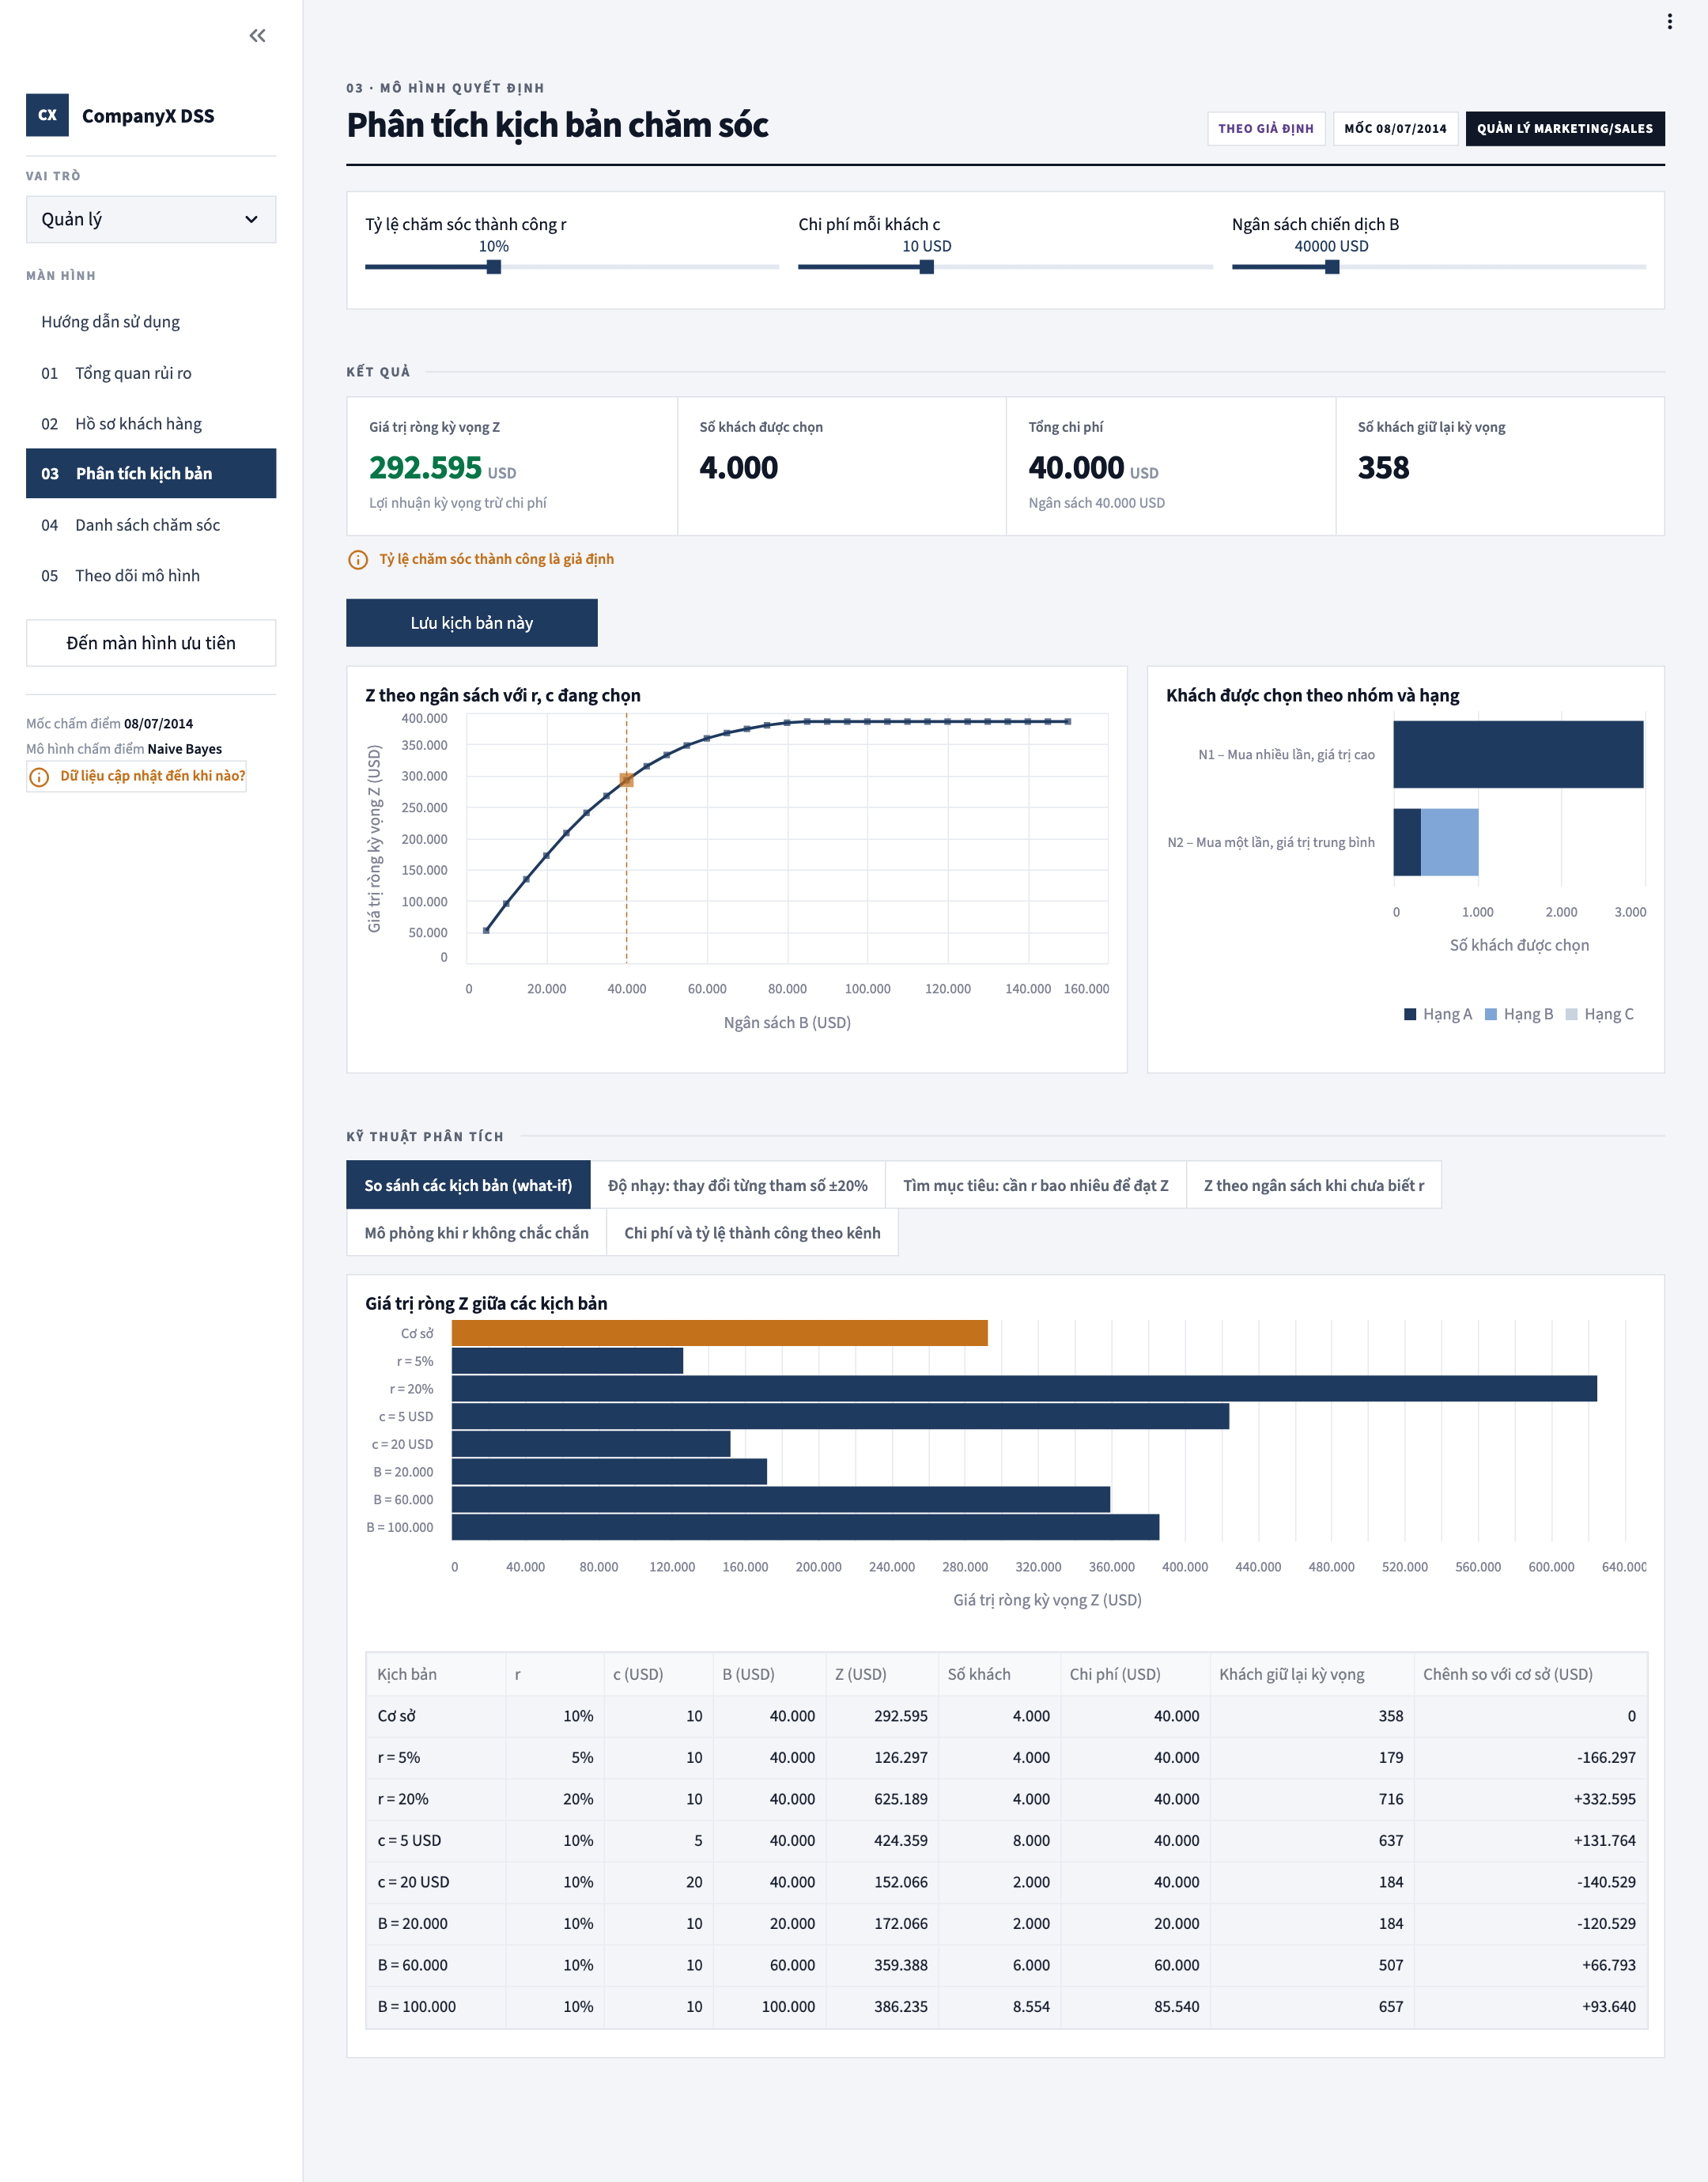
\includegraphics[width=0.95\textwidth]{d_man_hinh_3.png}
\caption{Màn hình 3: phân tích kịch bản và sự thay đổi giá trị ròng kỳ vọng trên DSS}
\label{fig:man3}
\end{figure}

\subsection{Khách thuộc nhóm nào}
Để người quản lý nắm cơ cấu khách và chọn cách chăm sóc phù hợp, DSS chia khách theo hai cách: hạng ABC theo giá trị và nhóm hành vi theo RFM. Cả hai tính tại mốc chấm điểm, chỉ dùng đơn trước mốc, không dùng nhãn. Nhóm và hạng không đổi danh sách chọn theo giá trị kỳ vọng, chúng dùng để mô tả trên dashboard và để chọn hình thức chăm sóc trong kho quy tắc. Kết quả ghi vào \texttt{analytics.\allowbreak CustomerSegment}, mô hình gom cụm lưu trong \texttt{analytics.\allowbreak ModelRegistry} và học lại cùng chu kỳ với mô hình phân lớp.

\subsubsection{Phân hạng ABC theo giá trị}
Phân tích ABC (mục~\ref{sec:rfmabc}) xếp khách theo Monetary (tổng \texttt{TotalDue} trước mốc) giảm dần rồi tính tỷ trọng luỹ kế:
\begin{equation}
    S_k = \frac{M_{(1)} + M_{(2)} + \dots + M_{(k)}}{\sum_i M_i} \label{eq:abc}
\end{equation}
Khách thứ $k$ thuộc hạng A nếu $S_{k-1} < 80\%$, hạng B nếu $80\% \leq S_{k-1} < 95\%$, còn lại là hạng C. Kết quả là 5.137 khách hạng A, 2.581 hạng B và 10.642 hạng C (Bảng~\ref{tab:abc}). Hạng B có xác suất không mua lại trung bình thấp nhất (0,665), hạng A ở giữa (0,749) và hạng C cao nhất (0,867). Mức rủi ro Cao tính theo phân vị trong từng hạng (Chương 5) cho 4.592 khách: hạng A 1.285, hạng B 646, hạng C 2.661. Ghép mức rủi ro với hạng ABC được ma trận Rủi ro $\times$ Giá trị trên dashboard, giúp nhìn cùng lúc nguy cơ và giá trị, ví dụ ô hạng A rủi ro Cao là nhóm cần xem trước khi lập chiến dịch.

\begin{table}[!htbp]
\centering
\caption{Phân hạng ABC theo Monetary tại mốc 08/07/2014}
\label{tab:abc}
\footnotesize
\begin{tabular}{lR{1.5cm}R{1.5cm}R{1.9cm}R{2.2cm}R{2.1cm}R{2.2cm}}
\toprule
Hạng & Số khách & Tỷ lệ khách & Tỷ trọng Monetary & Monetary trung vị (USD) & RiskScore trung bình & $v$ trung vị (USD) \\
\midrule
Hạng A & 5.137 & 28,0\% & 80\% & 4.859,51 & 0,749 & 938,42 \\
Hạng B & 2.581 & 14,1\% & 15\% & 1.918,26 & 0,665 & 493,38 \\
Hạng C & 10.642 & 58,0\% & 5\% & 71,01 & 0,867 & 20,56 \\
\bottomrule
\end{tabular}

\end{table}

Ngưỡng 80\%/95\% là quy ước, không tối ưu từ dữ liệu. Khi thử ngưỡng 70\%/90\% (Bảng~\ref{tab:abcnguong}), 2.278 khách đổi hạng nhưng danh sách theo kênh chỉ đổi từ 6.124 lên 6.480 khách và $Z$ giảm 1.802 USD (khoảng 0,7\%). Quyết định gần như không đổi nên nhóm giữ ngưỡng 80\%/95\%.

\begin{table}[!htbp]
\centering
\caption{Độ nhạy theo ngưỡng ABC: 80\%/95\% so với 70\%/90\%}
\label{tab:abcnguong}
\footnotesize
\begin{tabular}{lrr}
\toprule
Chỉ số & Ngưỡng 80\%/95\% (thiết kế) & Ngưỡng 70\%/90\% \\
\midrule
Số khách hạng A / B / C & 5.137 / 2.581 / 10.642 & 4.019 / 2.539 / 11.802 \\
Khách mức Cao hạng A / B / C & 1.285 / 646 / 2.661 & 1.005 / 635 / 2.951 \\
Khách đủ điều kiện R3 & 1.647 & 1.499 \\
Khách được chọn R3 / R5 & 983 / 5.141 & 934 / 5.546 \\
Tổng khách được chọn & 6.124 & 6.480 \\
Chi phí (USD) & 39.998 & 39.988 \\
$Z$ (USD) & 256.502 & 254.700 \\
Chênh $Z$ so với thiết kế (USD) & 0 & $-$1.802 \\
Số khách đổi hạng & 0 & 2.278 \\
\bottomrule
\end{tabular}

\end{table}

\subsubsection{Năm nhóm hành vi bằng K-means}
Nhóm chọn K-means~\cite{han2011} vì chạy nhanh với vài chục nghìn khách, mỗi nhóm có tâm nên dễ diễn giải, và khách mới được gán vào nhóm gần nhất mà không cần chạy lại. Đặc trưng là Recency, Frequency và Monetary tại mốc. Frequency và Monetary lệch phải mạnh nên lấy $\ln(1+x)$, rồi cả ba chuẩn hoá z-score để không đặc trưng nào lấn át khoảng cách. Thống kê Hopkins (đo mức dữ liệu tụ thành cụm, gần 0 là có cụm, 0,5 là phân bố ngẫu nhiên) bằng 0,004, cho thấy dữ liệu có cấu trúc cụm rõ. Số cụm chọn từ 2 đến 10 bằng đường Elbow và hệ số Silhouette~\cite{rousseeuw1987}, với yêu cầu số nhóm đủ ít để đặt tên và gắn quy tắc. Đường WCSS (tổng bình phương khoảng cách trong cụm) gãy trong khoảng $k=3$ đến 5, trong khoảng này $k=5$ có Silhouette cao nhất (0,466) (Bảng~\ref{tab:chonk}, Hình~\ref{fig:chonk}). Các $k$ lớn hơn có Silhouette nhỉnh hơn một chút nhưng nhóm nhỏ dần, nên nhóm chọn $k=5$. Kết quả ổn định: chỉ số Adjusted Rand Index~\cite{hubert1985} (đo mức giống nhau giữa hai cách chia nhóm, 1 là trùng khớp) bằng 1,0 với ba lần khởi tạo khác và 0,995 khi so với gom cụm phân cấp Ward.

\begin{table}[!htbp]
\centering
\caption{Chọn số cụm $k$: WCSS và Silhouette}
\label{tab:chonk}
\footnotesize
\begin{tabular}{crr}
\toprule
$k$ & WCSS & Silhouette \\
\midrule
2 & 34.456,1 & 0,412 \\
3 & 25.155,1 & 0,449 \\
4 & 18.689,9 & 0,409 \\
5 & 14.784,0 & 0,466 \\
6 & 12.019,8 & 0,452 \\
7 & 10.204,1 & 0,460 \\
8 & 8.517,2 & 0,471 \\
9 & 6.951,6 & 0,455 \\
10 & 5.878,5 & 0,481 \\
\bottomrule
\end{tabular}

\end{table}

\begin{figure}[!htbp]
\centering
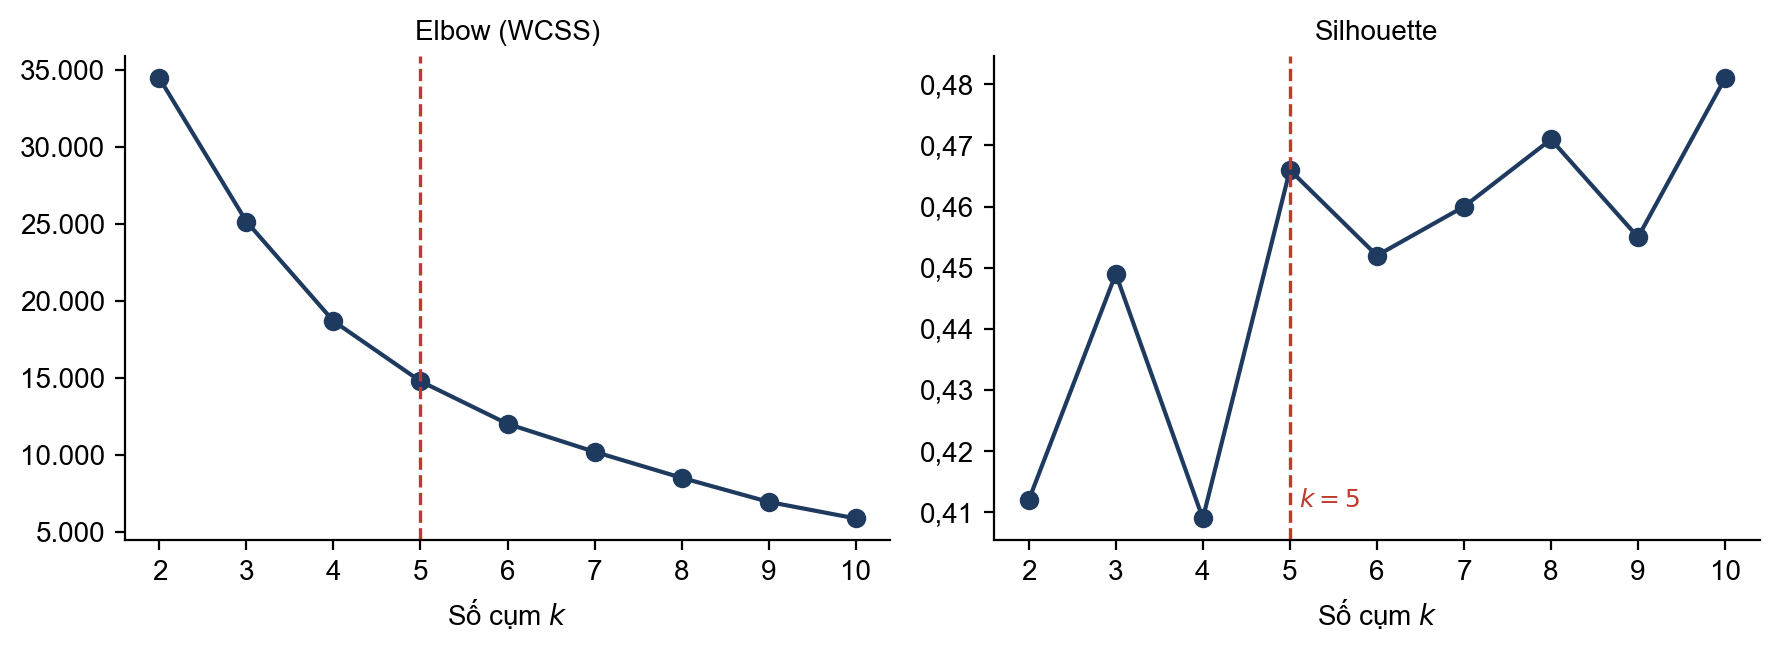
\includegraphics[width=0.8\textwidth]{d_chon_k.png}
\caption{Elbow và Silhouette khi chọn số cụm $k$}
\label{fig:chonk}
\end{figure}

Mỗi nhóm được đặt tên theo mức Recency, Frequency, Monetary so với các nhóm còn lại (Bảng~\ref{tab:honhom}).
\begin{itemize}
    \item \textbf{N1, mua nhiều lần, giá trị cao:} 4.926 khách (26,8\%), mua trung bình 2,2 lần, Monetary trung vị 4.910 USD, giữ 75,6\% tổng giá trị.
    \item \textbf{N2, mua một lần, giá trị trung bình:} 3.741 khách (20,4\%).
    \item \textbf{N3, mua một lần, đã lâu không quay lại:} 428 khách (2,3\%), Recency trung vị 917,5 ngày.
    \item \textbf{N4, mua lặp lại, giá trị thấp:} 1.839 khách (10,0\%), mua 2,7 lần nhưng chủ yếu là phụ kiện, Monetary trung vị chỉ 118 USD.
    \item \textbf{N5, mua một lần, giá trị thấp:} 7.426 khách (40,4\%), đông nhất, mua khoảng 44 USD.
\end{itemize}
N1 và N2 chiếm khoảng 93,6\% tổng Monetary. Hai dòng cuối của Bảng~\ref{tab:honhom} cho thấy nhóm nào được chọn chăm sóc. N4 và N5 không có khách nào $EV$ dương vì giá trị một lần mua quá nhỏ so với chi phí. N3 có 62,6\% khách $EV$ dương nhưng không khách nào được chọn ở ngân sách cơ sở, vì lợi trên mỗi USD thấp hơn các nhóm khác. Danh sách cuối chỉ gồm N1 (3.964 khách) và N2 (2.160 khách), đúng ý đồ dồn ngân sách vào khách có giá trị. Hình~\ref{fig:man1} là màn hình tổng quan trình bày các kết quả này.

\begin{table}[!htbp]
\centering
\caption{Hồ sơ năm nhóm khách hàng K-means tại mốc 08/07/2014}
\label{tab:honhom}
\footnotesize
\resizebox{\textwidth}{!}{\begin{tabular}{lrrrrr}
\toprule
Chỉ số & N1 & N2 & N3 & N4 & N5 \\
\midrule
Số khách & 4.926 & 3.741 & 428 & 1.839 & 7.426 \\
Tỷ lệ khách & 26,8\% & 20,4\% & 2,3\% & 10,0\% & 40,4\% \\
Recency trung vị (ngày) & 170 & 183 & 917,5 & 100 & 191 \\
Frequency trung bình & 2,21 & 1,00 & 1,00 & 2,66 & 1,00 \\
Monetary trung vị (USD) & 4.909,93 & 1.297,80 & 3.953,99 & 117,96 & 44,18 \\
Tỷ trọng Monetary & 75,6\% & 18,0\% & 4,3\% & 0,9\% & 1,3\% \\
Khách hạng A / B / C & 4.280 / 645 / 1 & 561 / 1.810 / 1.370 & 296 / 102 / 30 & 0 / 24 / 1.815 & 0 / 0 / 7.426 \\
RiskScore trung bình & 0,806 & 0,702 & 0,100 & 0,969 & 0,858 \\
Tỷ lệ mức Cao & 33,4\% & 7,0\% & 0,0\% & 55,2\% & 22,5\% \\
Tỷ lệ khách $EV>0$ & 98,7\% & 91,6\% & 62,6\% & 0,0\% & 0,0\% \\
Được chọn theo kênh & 3.964 & 2.160 & 0 & 0 & 0 \\
\bottomrule
\end{tabular}
}
\end{table}

\begin{figure}[!htbp]
\centering
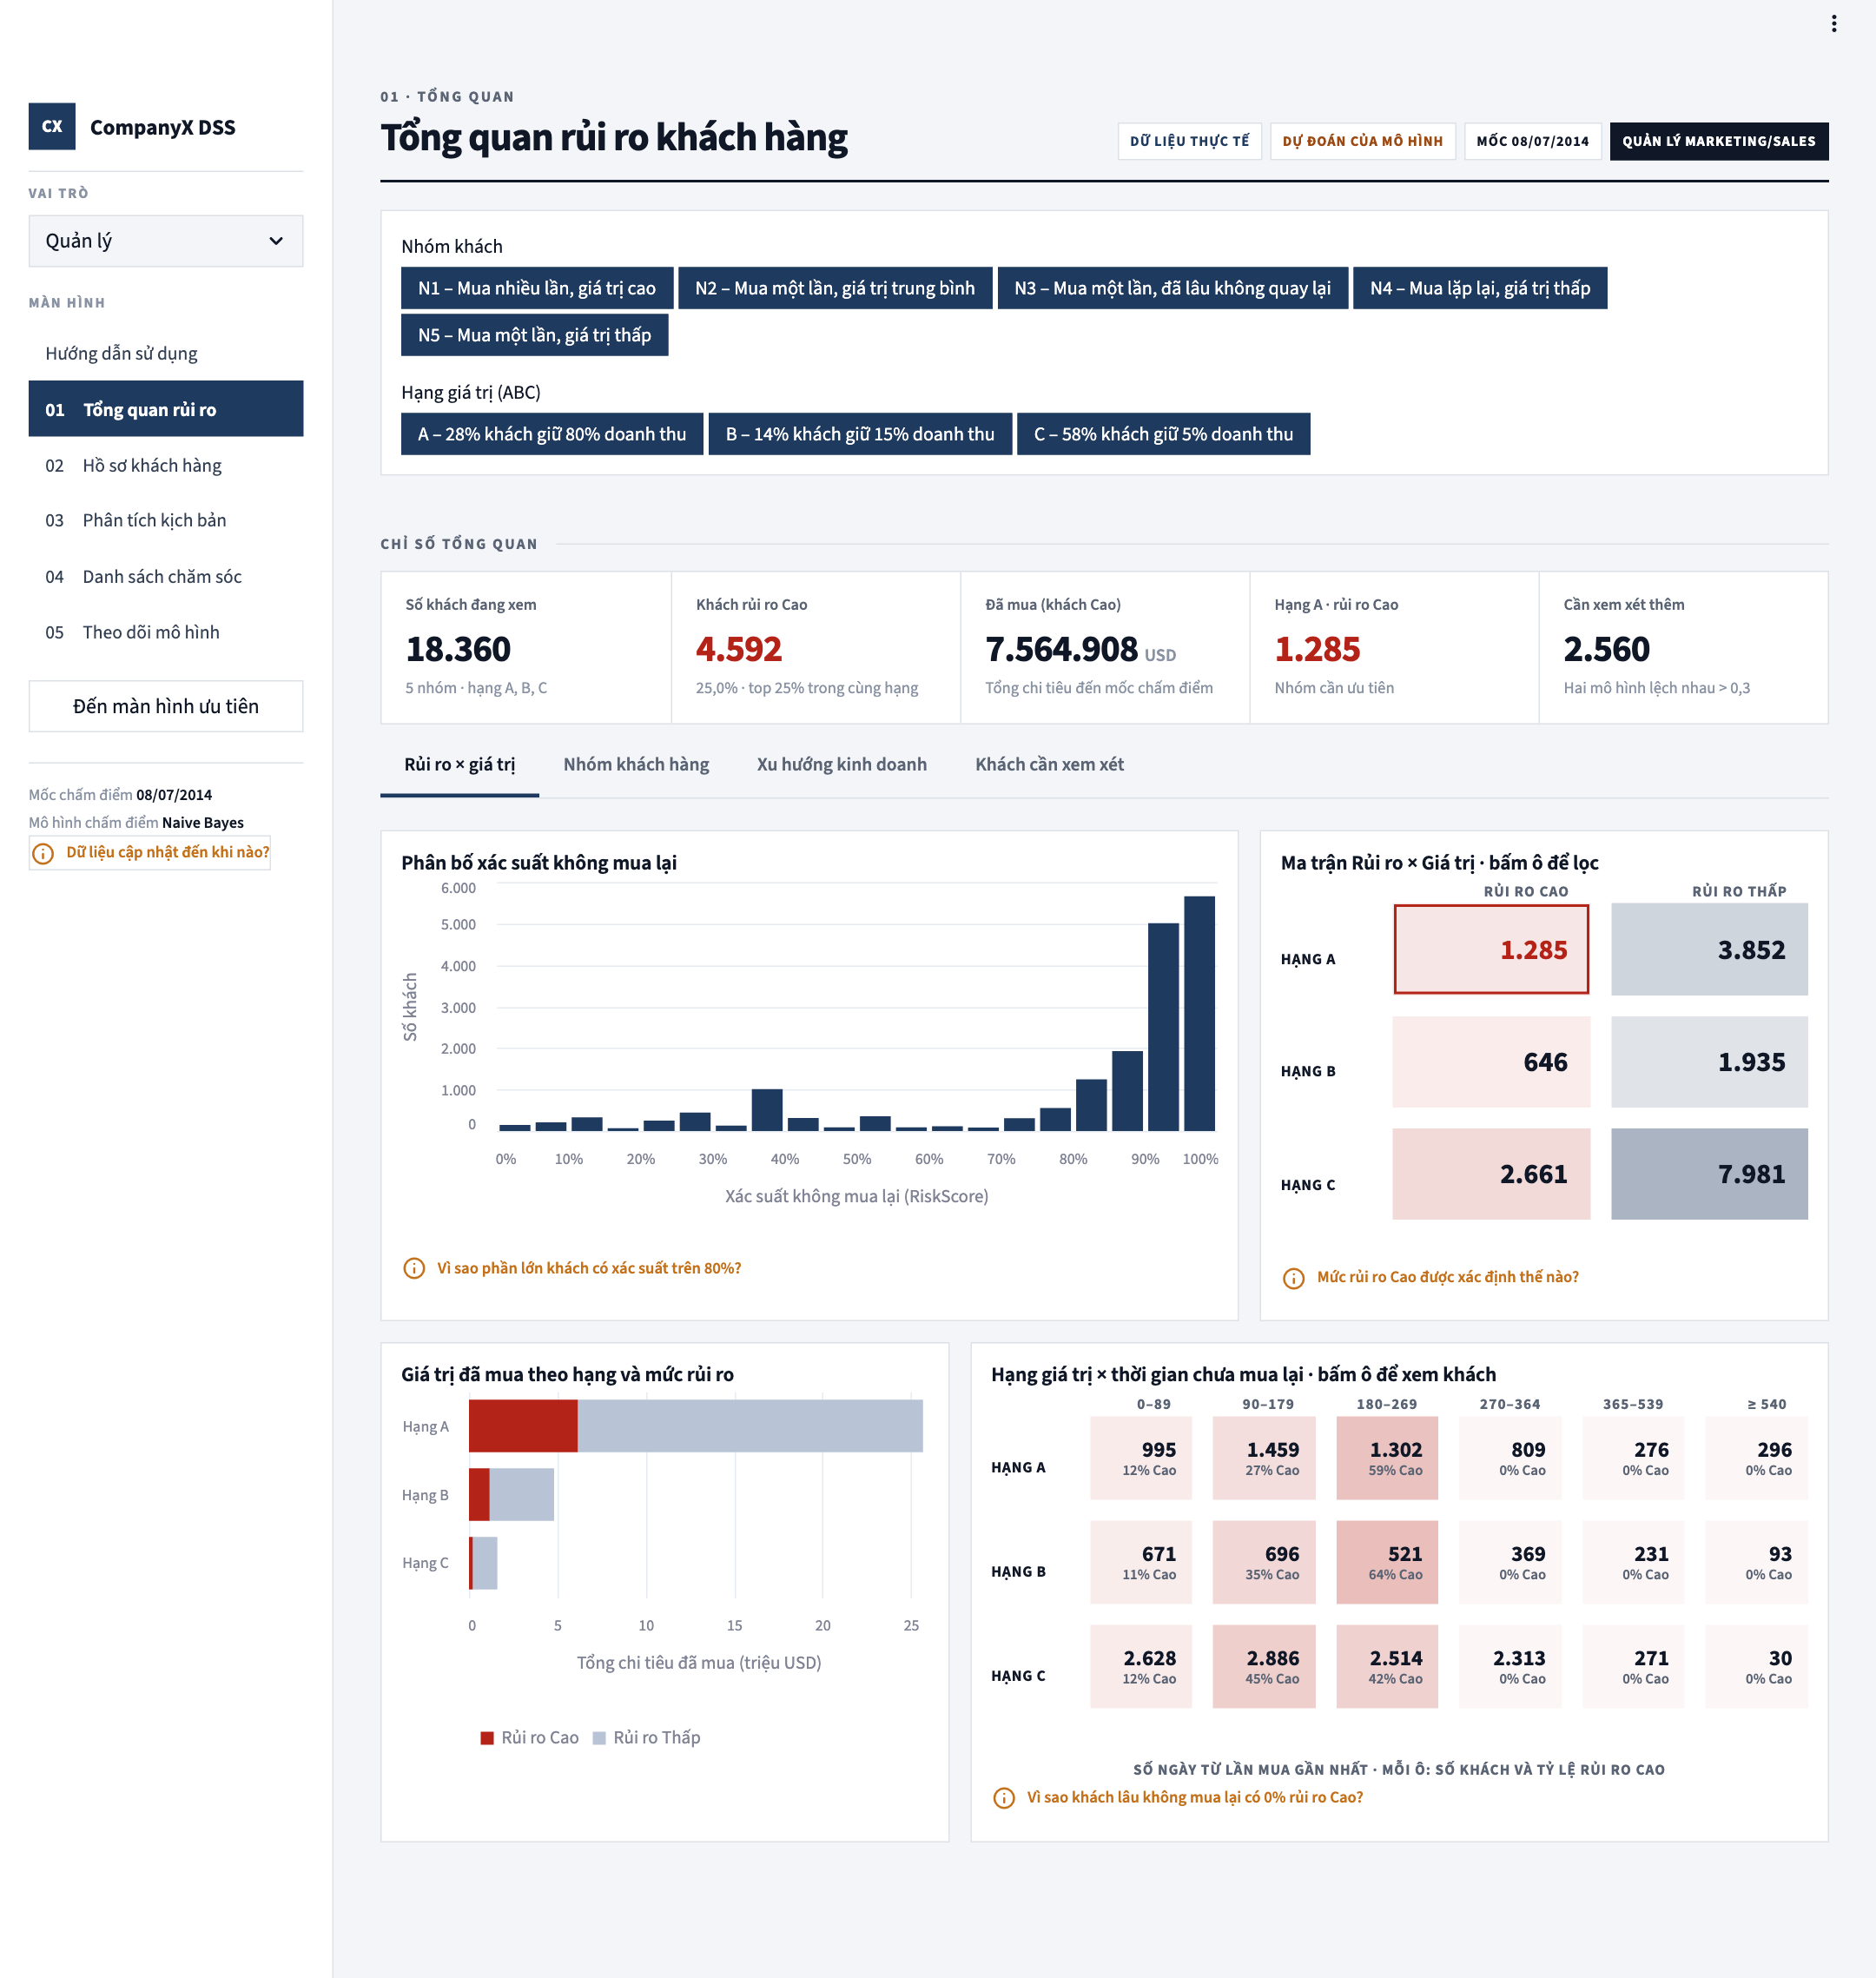
\includegraphics[width=0.95\textwidth]{d_man_hinh_1.png}
\caption{Màn hình 1: tổng quan rủi ro và phân bố khách hàng theo hạng giá trị}
\label{fig:man1}
\end{figure}

\subsection{Chăm sóc bằng cách nào: kho quy tắc}
\subsubsection{Kho quy tắc và trình tự áp dụng}
Phân hệ tri thức lưu các quy tắc IF--THEN để loại khách không đủ điều kiện, gán hình thức liên hệ, đề xuất sản phẩm và giải thích vì sao có đề xuất. Tri thức đến từ ba nguồn: từ dữ liệu (hồ sơ nhóm, cơ cấu sản phẩm, luật kết hợp), từ mô hình (\texttt{RiskScore}, \texttt{RiskLevel}, \texttt{TopFactors} là luật của lá cây mà khách rơi vào, giá trị kỳ vọng) và từ người quản lý (chính sách chăm sóc, mức ưu đãi, kênh liên hệ). Kho gồm chín quy tắc R1 đến R9 (Bảng~\ref{tab:luat}), lưu theo phiên bản tại \texttt{analytics.\allowbreak CareRule}. Bảy quy tắc đang bật. R1 và R9 cần nhật ký liên hệ và kết quả chiến dịch nên đã thiết kế nhưng còn tắt.

\begin{table}[!htbp]
\centering
\caption{Kho quy tắc chăm sóc R1 đến R9}
\label{tab:luat}
\footnotesize
\begin{tabular}{p{0.8cm}p{2.5cm}p{4.8cm}p{4.2cm}p{1.6cm}}
\toprule
Mã & Loại & Điều kiện & Hành động & Trạng thái \\
\midrule
R1 & Loại trừ & Khách đã được liên hệ trong 90 ngày trước (nhật ký CRM) & Không đưa vào danh sách mới & Tắt, thiếu dữ liệu CRM \\
R2 & Loại trừ & $p \cdot r \cdot v - c \leq 0$ & Không đưa vào danh sách chăm sóc cá nhân & Bật \\
R3 & Hình thức liên hệ & Nhóm N1 và mức rủi ro Cao & Liên hệ cá nhân kèm ưu đãi (25 USD, thành công 15\%) & Bật \\
R4 & Hình thức liên hệ & Nhóm N3 & Nội dung mời quay lại kèm ưu đãi (15 USD, thành công 12\%) & Bật \\
R5 & Hình thức liên hệ & Các trường hợp còn lại & Email cá nhân hoá gửi tự động (3 USD, thành công 5\%) & Bật \\
R6 & Sản phẩm gợi ý & Đã mua Touring Bikes, chưa mua Helmets & Gợi ý Helmets & Bật \\
R7 & Sản phẩm gợi ý & Đã mua Mountain Bikes, chưa mua Fenders & Gợi ý Fenders & Bật \\
R8 & Sản phẩm gợi ý & Đã mua Gloves chưa mua Helmets, hoặc đã mua Hydration Packs chưa mua Bottles and Cages & Gợi ý Helmets hoặc Bottles and Cages tương ứng & Bật \\
R9 & Giám sát mô hình & Đã đủ nhãn 90 ngày sau chiến dịch & So ROC-AUC với Recency trên nhóm đối chứng, cảnh báo nếu không hơn & Tắt, thiếu dữ liệu CRM \\
\bottomrule
\end{tabular}
\end{table}

Hình~\ref{fig:luongquytac} là trình tự áp dụng. Quy tắc hình thức liên hệ (R3 đến R5) chạy trước bước tối ưu: mỗi khách được gán một hình thức kèm chi phí và tỷ lệ thành công, rồi R2 và bài toán tối ưu chọn khách trong ngân sách. Quy tắc sản phẩm (R6 đến R8) chỉ áp dụng cho khách đã chọn, khách không khớp quy tắc nào nhận lời mời quay lại kèm giới thiệu chung các nhóm phụ kiện. Mỗi khuyến nghị kèm mã quy tắc đã kích hoạt, căn cứ của quy tắc và \texttt{TopFactors} của khách, và được lưu vào \texttt{analytics.\allowbreak CareRecommendation}. Người quản lý có thể thêm, sửa hoặc tắt quy tắc, mỗi thay đổi tạo một phiên bản mới có ngày hiệu lực và người cập nhật.

\begin{figure}[!htbp]
\centering
\begin{tikzpicture}[
  box/.style={draw, rounded corners=2pt, text width=10.5cm, minimum height=0.9cm, align=center, font=\small},
  off/.style={draw, dashed, rounded corners=2pt, text width=10.5cm, minimum height=0.9cm, align=center, font=\small},
  cert/.style={-{Stealth[length=2mm]}}, node distance=0.55cm]
  \node[box] (a) {Khách tại mốc chấm điểm: \texttt{RiskScore}, nhóm, hạng ABC, $v_i$};
  \node[off, below=of a] (b) {\textbf{R1} loại khách đã được liên hệ trong 90 ngày trước (cần nhật ký CRM)};
  \node[box, below=of b] (c) {\textbf{R3 đến R5} gán hình thức liên hệ kèm chi phí $c_k$ và tỷ lệ thành công $r_k$};
  \node[box, below=of c] (d) {\textbf{R2} loại khách có $EV_i \leq 0$};
  \node[box, below=of d] (e) {Tối ưu: chọn khách trong ngân sách $B$ (bài toán cái túi 0--1)};
  \node[box, below=of e] (f) {\textbf{R6 đến R8} gợi ý sản phẩm cho khách được chọn (nội dung mặc định nếu không khớp)};
  \node[box, below=of f] (g) {Danh sách chăm sóc kèm giải thích: mã quy tắc đã kích hoạt, căn cứ, \texttt{TopFactors}};
  \node[off, below=of g] (h) {\textbf{R9} giám sát mô hình sau chiến dịch (cần nhóm đối chứng và dữ liệu CRM)};
  \foreach \s/\t in {a/b,b/c,c/d,d/e,e/f,f/g}{\draw[cert] (\s) -- (\t);}
  \draw[cert, dashed] (g) -- (h);
\end{tikzpicture}

\caption{Trình tự áp dụng quy tắc và mô hình khi tạo danh sách chăm sóc}
\label{fig:luongquytac}
\end{figure}

\subsubsection{Gợi ý sản phẩm bằng luật kết hợp}
N1, N2 và N3 gần như chỉ mua xe đạp, còn N4 và N5 không mua xe và 73\% đến 77\% giá trị là phụ kiện (Bảng~\ref{tab:cocausp}). Vì vậy gợi ý cho N1 và N2 nên là phụ kiện đi kèm xe. Luật kết hợp (support, confidence và lift như ở Chương 2) tìm bằng Apriori~\cite{han2011} trên 18.360 giỏ theo khách với 17 nhóm sản phẩm nhỏ mà khách cá nhân từng mua, mỗi giỏ là tập nhóm sản phẩm khách đã mua trước mốc. Nhóm tính theo khách thay vì theo đơn vì mục đích là gợi ý món khách chưa từng mua, không phải gợi ý mua kèm tại quầy. Ngưỡng support 1\% (khoảng 184 khách) để luật có đủ số khách, confidence 20\% để cứ 5 khách mua vế trái có 1 khách mua vế phải, và lift phải lớn hơn 1. Từ 164 luật, nhóm giữ 26 luật có một mục mỗi vế và vế phải là phụ kiện hoặc quần áo. Bảng~\ref{tab:apriori} liệt kê 10 luật có lift cao nhất.

\begin{table}[!htbp]
\centering
\caption{Cơ cấu sản phẩm theo nhóm}
\label{tab:cocausp}
\footnotesize
\begin{tabular}{lrrrrr}
\toprule
Nhóm & Bikes & Accessories & Clothing & Tỷ lệ đã mua xe & NSub trung bình \\
\midrule
N1 & 98,6\% & 0,9\% & 0,5\% & 100,0\% & 3,33 \\
N2 & 96,2\% & 2,5\% & 1,3\% & 99,9\% & 2,31 \\
N3 & 100,0\% & 0,0\% & 0,0\% & 100,0\% & 1,00 \\
N4 & 0,0\% & 73,1\% & 26,9\% & 0,0\% & 3,23 \\
N5 & 0,0\% & 77,3\% & 22,7\% & 0,0\% & 1,74 \\
\bottomrule
\end{tabular}

\end{table}

\begin{table}[!htbp]
\centering
\caption{Luật kết hợp dùng làm gợi ý sản phẩm (10 trong 26 luật, xếp theo lift)}
\label{tab:apriori}
\footnotesize
\begin{tabular}{clllrr}
\toprule
Hạng & Vế trái & Vế phải & Support & Confidence & Lift \\
\midrule
1 & Shorts & Caps & 1,36\% & 24,7\% & 2,15 \\
2 & Shorts & Jerseys & 2,03\% & 36,8\% & 2,13 \\
3 & Hydration Packs & Bottles and Cages & 1,92\% & 49,9\% & 2,03 \\
4 & Mountain Bikes & Fenders & 4,85\% & 21,9\% & 1,92 \\
5 & Bike Stands & Tires and Tubes & 1,14\% & 87,5\% & 1,91 \\
6 & Caps & Jerseys & 3,70\% & 32,3\% & 1,87 \\
7 & Jerseys & Caps & 3,70\% & 21,5\% & 1,87 \\
8 & Gloves & Jerseys & 2,06\% & 27,8\% & 1,61 \\
9 & Gloves & Helmets & 3,71\% & 49,9\% & 1,55 \\
10 & Touring Bikes & Helmets & 5,69\% & 49,3\% & 1,53 \\
\bottomrule
\end{tabular}

\end{table}

Trước khi chạy Apriori, nhóm đặt năm luật ứng viên theo lý do nghiệp vụ: Touring Bikes $\rightarrow$ Helmets và Touring Bikes $\rightarrow$ Bottles and Cages (xe đường dài cần mũ và nước), Mountain Bikes $\rightarrow$ Fenders (đường bùn cần chắn bùn), Gloves $\rightarrow$ Helmets (đồ bảo hộ mua cùng nhau) và Hydration Packs $\rightarrow$ Bottles and Cages (cùng nhóm đựng nước). Cả năm đều có trong 26 luật gợi ý (Bảng~\ref{tab:apriori_dc}), bốn luật được đưa vào ba quy tắc R6, R7 và R8 (R8 gộp hai luật), luật Touring Bikes $\rightarrow$ Bottles and Cages chỉ dùng để kiểm tra, chưa đưa vào kho. Khi tính lại theo từng đơn (27.382 đơn), cả năm luật vẫn có lift lớn hơn 1, riêng Mountain Bikes $\rightarrow$ Fenders có confidence theo đơn dưới 20\% nên chỉ mạnh khi xét theo khách. Hai luật mạnh chưa dùng là Shorts $\rightarrow$ Caps và Shorts $\rightarrow$ Jerseys, có thể thêm ở phiên bản sau. Luật kết hợp chỉ mô tả các sản phẩm xuất hiện cùng nhau, không cho biết thứ tự mua hay nhân quả, nên chỉ dùng để chọn sản phẩm nêu trong nội dung chăm sóc, không dùng để chọn khách.

\begin{table}[!htbp]
\centering
\caption{Năm luật ứng viên và vị trí trong kết quả Apriori}
\label{tab:apriori_dc}
\footnotesize
\begin{tabular}{lp{4.6cm}R{1.9cm}R{1.9cm}R{2.1cm}R{1.9cm}}
\toprule
Quy tắc & Luật & Lift theo khách & Hạng trong 26 luật & Confidence theo đơn & Lift theo đơn \\
\midrule
R6 & Touring Bikes $\rightarrow$ Helmets & 1,53 & 10 & 41,2\% & 1,77 \\
R6b & Touring Bikes $\rightarrow$ Bottles and Cages & 1,47 & 12 & 25,5\% & 1,48 \\
R7 & Mountain Bikes $\rightarrow$ Fenders & 1,92 & 4 & 18,1\% & 2,35 \\
R8 & Gloves $\rightarrow$ Helmets & 1,55 & 9 & 42,0\% & 1,80 \\
R8b & Hydration Packs $\rightarrow$ Bottles and Cages & 2,03 & 3 & 45,3\% & 2,63 \\
\bottomrule
\end{tabular}

\end{table}

\subsubsection{Danh sách chăm sóc theo kênh}
Khi mỗi khách được gán một kênh $k(i)$ với chi phí $c_k$ và tỷ lệ thành công $r_k$ riêng theo R3 đến R5, bài toán thành $\max \sum_i x_i (p_i\, r_{k(i)}\, v_i - c_{k(i)})$ với ràng buộc $\sum_i x_i\, c_{k(i)} \leq B$. DSS giải bằng quy hoạch nguyên, thuật toán tham lam xếp theo lợi trên mỗi USD chi phí cho cùng lời giải. Với ngân sách 40.000 USD, DSS chọn 6.124 khách, chi 39.998 USD và đạt $Z = 256.502$ USD (Bảng~\ref{tab:theokenh}, tổng EV các dòng chênh 1 USD so với $Z$ do làm tròn), cao hơn 6,9\% so với cách xếp theo $p \cdot v$ mà bỏ qua chi phí kênh. Khi ngân sách có hạn, cách chọn đúng là xếp theo lợi trên mỗi USD chứ không phải chọn mọi khách có $EV$ dương. Kênh R4 chỉ bắt đầu có khách khi ngân sách từ khoảng 61.213 USD, nên muốn chăm sóc nhóm N3 thì phải tăng ngân sách đến mức đó. Phương án theo kênh và kịch bản cơ sở (4.000 khách, $Z$ 292.595 USD) dùng giả định chi phí và tỷ lệ thành công khác nhau nên không so trực tiếp $Z$ để kết luận phương án nào tốt hơn. Màn hình 4 (Hình~\ref{fig:man4}) trình bày danh sách này kèm nhật ký điều chỉnh và nút xuất CSV.

\begin{table}[!htbp]
\centering
\caption{Danh sách chăm sóc theo kênh}
\label{tab:theokenh}
\footnotesize
\begin{tabular}{lrrrr}
\toprule
Kênh & Khách đủ điều kiện & Được chọn & Chi phí (USD) & EV tổng (USD) \\
\midrule
R3 & 1.647 & 983 & 24.575 & 112.109 \\
R4 & 428 & 0 & 0 & 0 \\
R5 & 16.285 & 5.141 & 15.423 & 144.392 \\
Tổng & 18.360 & 6.124 & 39.998 & 256.501 \\
\bottomrule
\end{tabular}

\end{table}

\begin{figure}[!htbp]
\centering
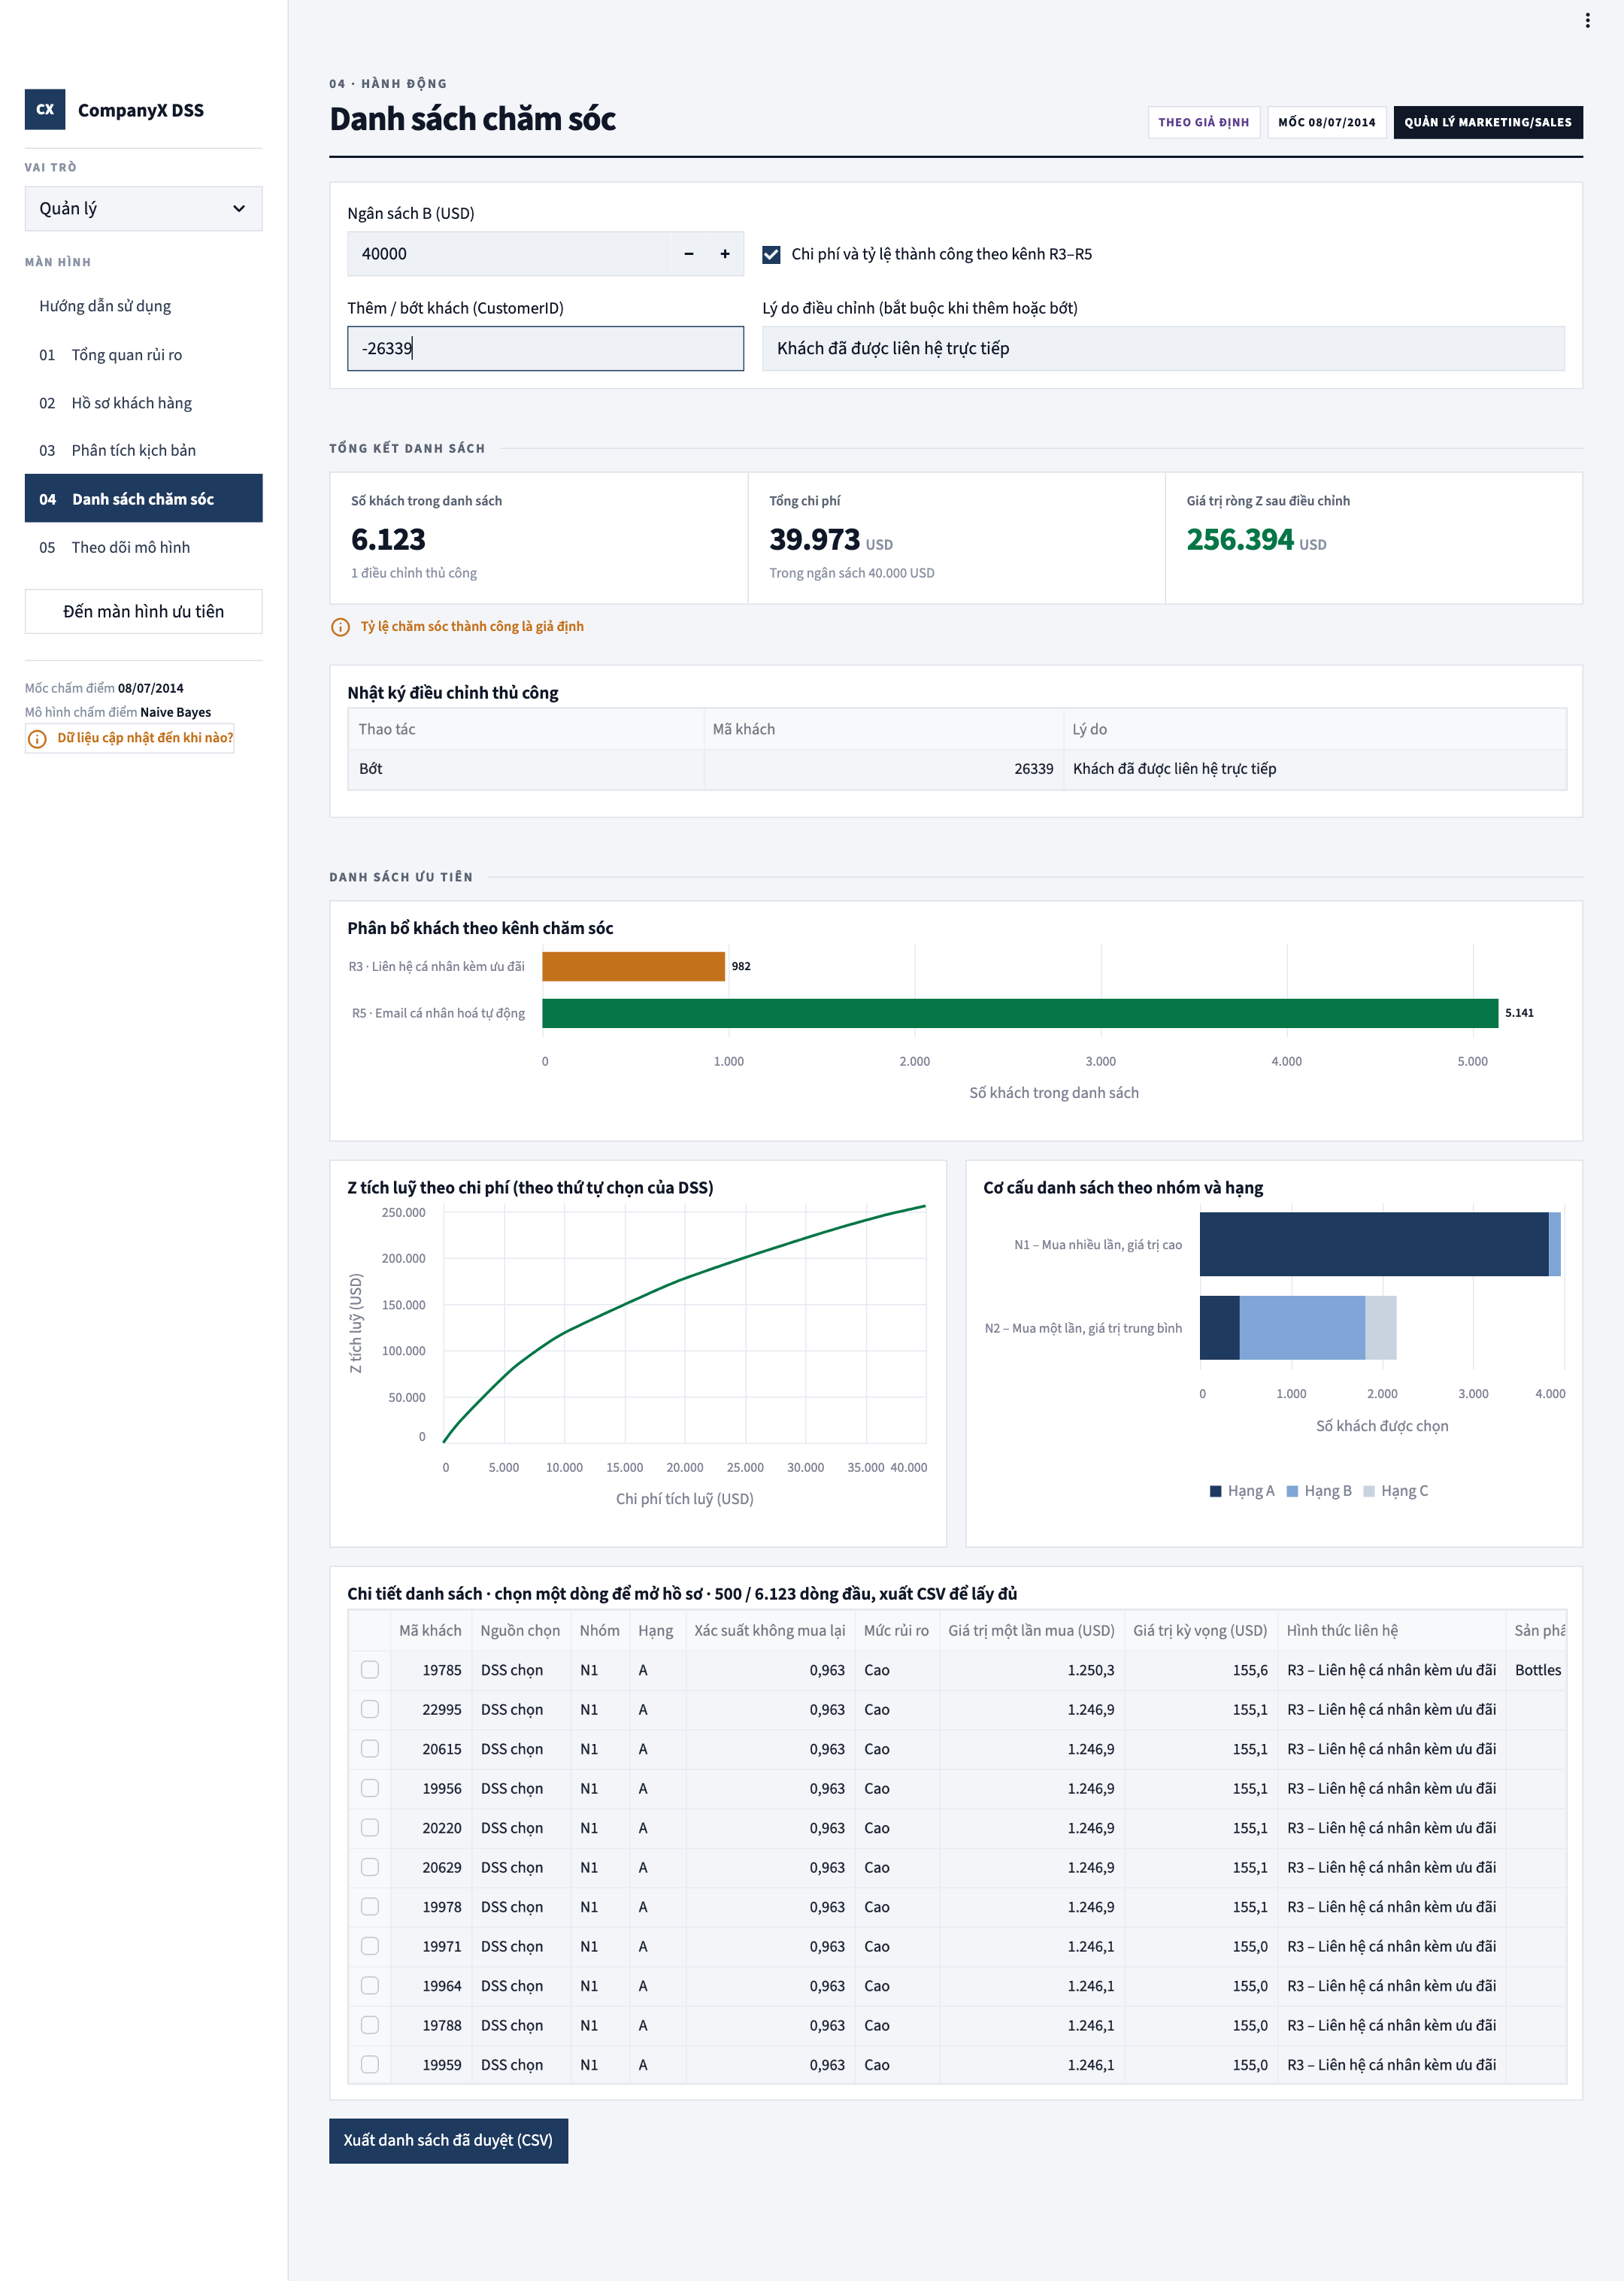
\includegraphics[width=0.95\textwidth]{d_man_hinh_4.png}
\caption{Màn hình 4: danh sách khách hàng ưu tiên chăm sóc sau khi điều chỉnh}
\label{fig:man4}
\end{figure}

\subsection{Ngân sách bao nhiêu khi chưa biết tỷ lệ thành công}
Tỷ lệ thành công $r$ chưa đo được vì chưa có chiến dịch nào. Mục này cho người quản lý thấy $Z$ phụ thuộc vào $r$ đến đâu và đặt ngân sách theo mức chấp nhận rủi ro của mình. Mọi giá trị $Z$ đều là kỳ vọng theo giả định.

\subsubsection{Độ nhạy và tìm mục tiêu}
Thay từng tham số $r$, $p$, $g$, $c$, $B$ quanh kịch bản cơ sở $\pm 20\%$ (Bảng~\ref{tab:donhay_b}, Hình~\ref{fig:donhay}). $r$ và $g$ cùng làm $Z$ đổi $\pm 22{,}7\%$ vì nhân với nhau trong doanh thu, còn $c$ và $B$ tác động ít hơn vì chỉ thêm hoặc bớt khách cuối danh sách. Trong các tham số nhân, $g$ đo được từ dữ liệu, $p$ ước lượng bằng mô hình, còn $r$ chưa có dữ liệu nên cần đo trước tiên~\cite{lemmens2020}.

\begin{table}[!htbp]
\centering
\caption{Độ nhạy của $Z$ khi từng tham số thay đổi 20\%}
\label{tab:donhay_b}
\footnotesize
\resizebox{\textwidth}{!}{\begin{tabular}{lrrrr}
\toprule
Tham số & $Z$ khi giảm 20\% (USD) & Chênh & $Z$ khi tăng 20\% (USD) & Chênh \\
\midrule
$r$ & 226.076 & $-$22,7\% & 359.114 & +22,7\% \\
$p$ & 226.076 & $-$22,7\% & 327.591 & +12,0\% \\
$g$ (qua $v$) & 226.076 & $-$22,7\% & 359.114 & +22,7\% \\
$c$ & 342.856 & +17,2\% & 251.887 & $-$13,9\% \\
$B$ & 251.405 & $-$14,1\% & 326.198 & +11,5\% \\
\bottomrule
\end{tabular}
}
\end{table}

\begin{figure}[!htbp]
\centering
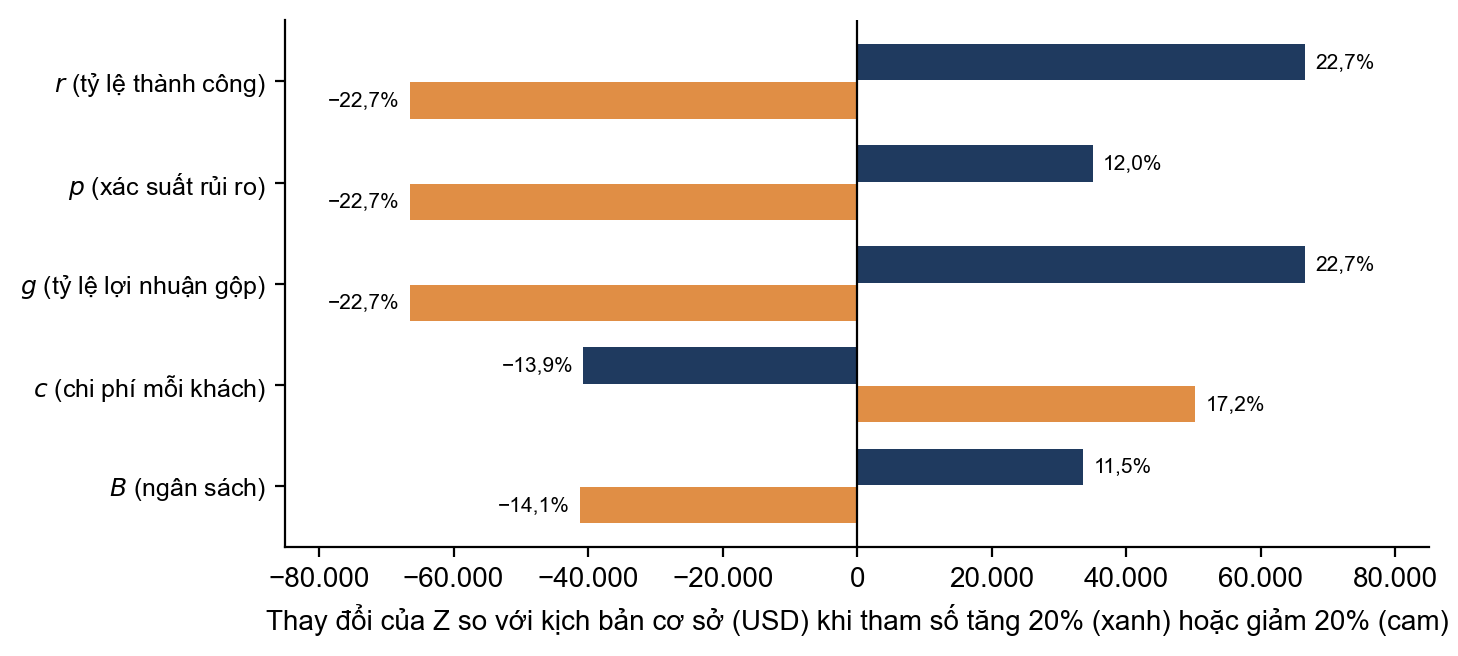
\includegraphics[width=0.8\textwidth]{d_do_nhay.png}
\caption{Thay đổi của $Z$ khi từng tham số của kịch bản cơ sở tăng hoặc giảm 20\%}
\label{fig:donhay}
\end{figure}

Tìm mục tiêu trả lời câu hỏi ngược: $r$ phải bằng bao nhiêu để $Z$ đạt mức $Z^*$. Với danh sách $K$ khách đã chốt, $Z$ là hàm bậc nhất của $r$ nên
\begin{equation}
    r^* = \frac{Z^* + c\,K}{\sum_{i=1}^{K} p_i\, v_i} \label{eq:rstar}
\end{equation}
Mức $r$ hoà vốn ($Z^*=0$) là 1,20\%, mức để $Z$ đạt 100.000 USD là 4,21\%. Chiến dịch chỉ lỗ khi tỷ lệ thành công thật dưới khoảng 1,2\%.

\subsubsection{Ba tiêu chí ra quyết định và mô phỏng}
Khi $r$ chưa biết, phương án là mức ngân sách $B$ và trạng thái là ba mức $r$: 2\% (bi quan), 10\% (cơ sở) và 20\% (lạc quan) với xác suất giả định 30\%, 50\% và 20\%. Gọi $Z(B,s)$ là giá trị ròng của phương án $B$ ở trạng thái $s$, ba tiêu chí ở Chương 2 là:
\begin{align}
    \text{Lạc quan:}\quad & B^* = \arg\max_B \left[\max_s Z(B,s)\right] \label{eq:lacquan}\\
    \text{Bi quan:}\quad & B^* = \arg\max_B \left[\min_s Z(B,s)\right] \label{eq:biquan}\\
    \text{Giá trị kỳ vọng:}\quad & B^* = \arg\max_B \sum_s P(s)\, Z(B,s) \label{eq:kyvong}
\end{align}
Bảng~\ref{tab:payoff} là $Z$ theo ngân sách và $r$. Người lạc quan và tiêu chí giá trị kỳ vọng chọn $B = 100.000$ USD, người bi quan chọn $B = 40.000$ USD. DSS không chọn thay người quản lý mà đưa ra phương án cho từng phong cách ra quyết định.

\begin{table}[!htbp]
\centering
\caption{$Z$ theo ngân sách và tỷ lệ chăm sóc thành công (USD)}
\label{tab:payoff}
\footnotesize
\resizebox{\textwidth}{!}{\begin{tabular}{rrrrrr}
\toprule
Ngân sách $B$ (USD) & Số khách & $r=2\%$ & $r=10\%$ & $r=20\%$ & Giá trị kỳ vọng \\
\midrule
20.000 & 2.000 & 18.413 & 172.066 & 364.132 & 164.383 \\
40.000 & 4.000 & 26.519 & 292.595 & 625.189 & 279.291 \\
60.000 & 6.000 & 23.878 & 359.388 & 778.775 & 342.612 \\
100.000 & 8.554 & 8.815 & 386.235 & 858.009 & 367.364 \\
\bottomrule
\end{tabular}
}
\end{table}

Thay cho ba mức rời rạc, mô phỏng coi $r$ là đại lượng ngẫu nhiên theo phân phối Beta (phân phối cho đại lượng từ 0 đến 1) với $\alpha=2{,}2$, $\beta=19{,}8$, trung bình 10\%, các $r_k$ theo kênh co giãn cùng hệ số. Mỗi lần mô phỏng rút một giá trị $r$ rồi tính $Z$ cho danh sách đã chốt, lặp 10.000 lần~\cite{turban2011}. Mô hình được kiểm định bằng cách tại $r=10\%$ kết quả phải trùng kịch bản cơ sở. Kết quả (Hình~\ref{fig:mophong}): $r$ trung bình 9,9\%, $Z$ trung bình 290.490 USD và xác suất lỗ 1,7\%. Xác suất này đúng theo phân phối giả định, không phải xác suất lỗ đã xác thực.

\begin{figure}[!htbp]
\centering
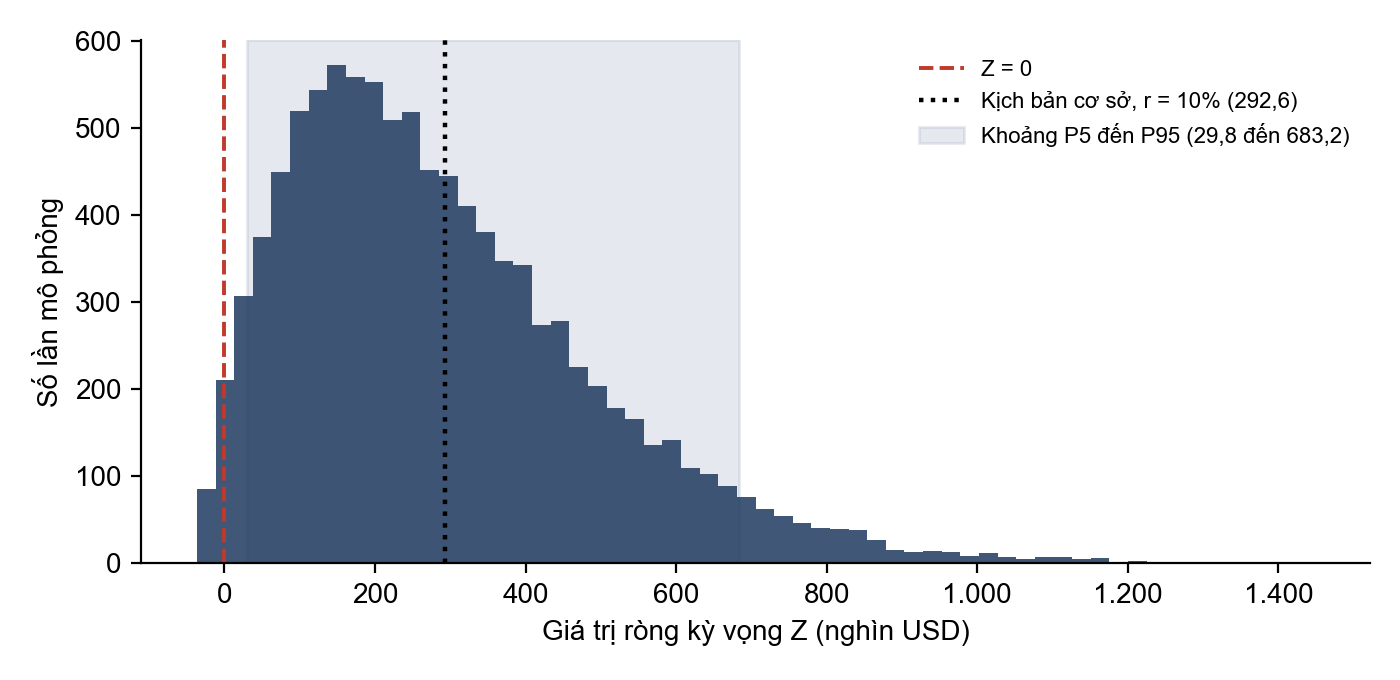
\includegraphics[width=0.7\textwidth]{d_mo_phong.png}
\caption{Phân bố của $Z$ trong 10.000 lần mô phỏng với $r$ theo phân phối Beta}
\label{fig:mophong}
\end{figure}

\subsubsection{Dự báo theo tháng}
Để ước quy mô kỳ 90 ngày khi đặt ngân sách và để cảnh báo khi thực tế lệch xa dự báo, màn hình theo dõi (Hình~\ref{fig:man5}) dùng hồi quy tuyến tính~\cite{han2011} trên chuỗi tháng của số đơn và doanh thu, với biến xu hướng và biến chỉ thị tháng. MAPE (sai số phần trăm tuyệt đối trung bình) ở hai tháng ngoài mẫu (tháng 4 và 5/2014) là 8,2\% với số đơn và 15,4\% với doanh thu, tốt hơn nhiều so với mức nền cùng tháng năm trước (84,9\% và 70,1\%) (Bảng~\ref{tab:dubao}). Tháng 6/2014 lệch mạnh vì không có đơn xe đạp, đúng là tình huống bất thường mà chức năng này cần phát hiện.

\begin{table}[!htbp]
\centering
\caption{Dự báo hồi quy tuyến tính số đơn và doanh thu}
\label{tab:dubao}
\footnotesize
\resizebox{\textwidth}{!}{\begin{tabular}{lrrr}
\toprule
Chỉ số & MAPE tháng 4--5/2014 & MAPE mức nền (cùng tháng năm trước) & Dự báo vượt thực tế tháng 6/2014 \\
\midrule
Số đơn & 8,2\% & 84,9\% & 134\% \\
Doanh thu & 15,4\% & 70,1\% & 3.721\% \\
\bottomrule
\end{tabular}
}
\end{table}

\begin{figure}[!htbp]
\centering
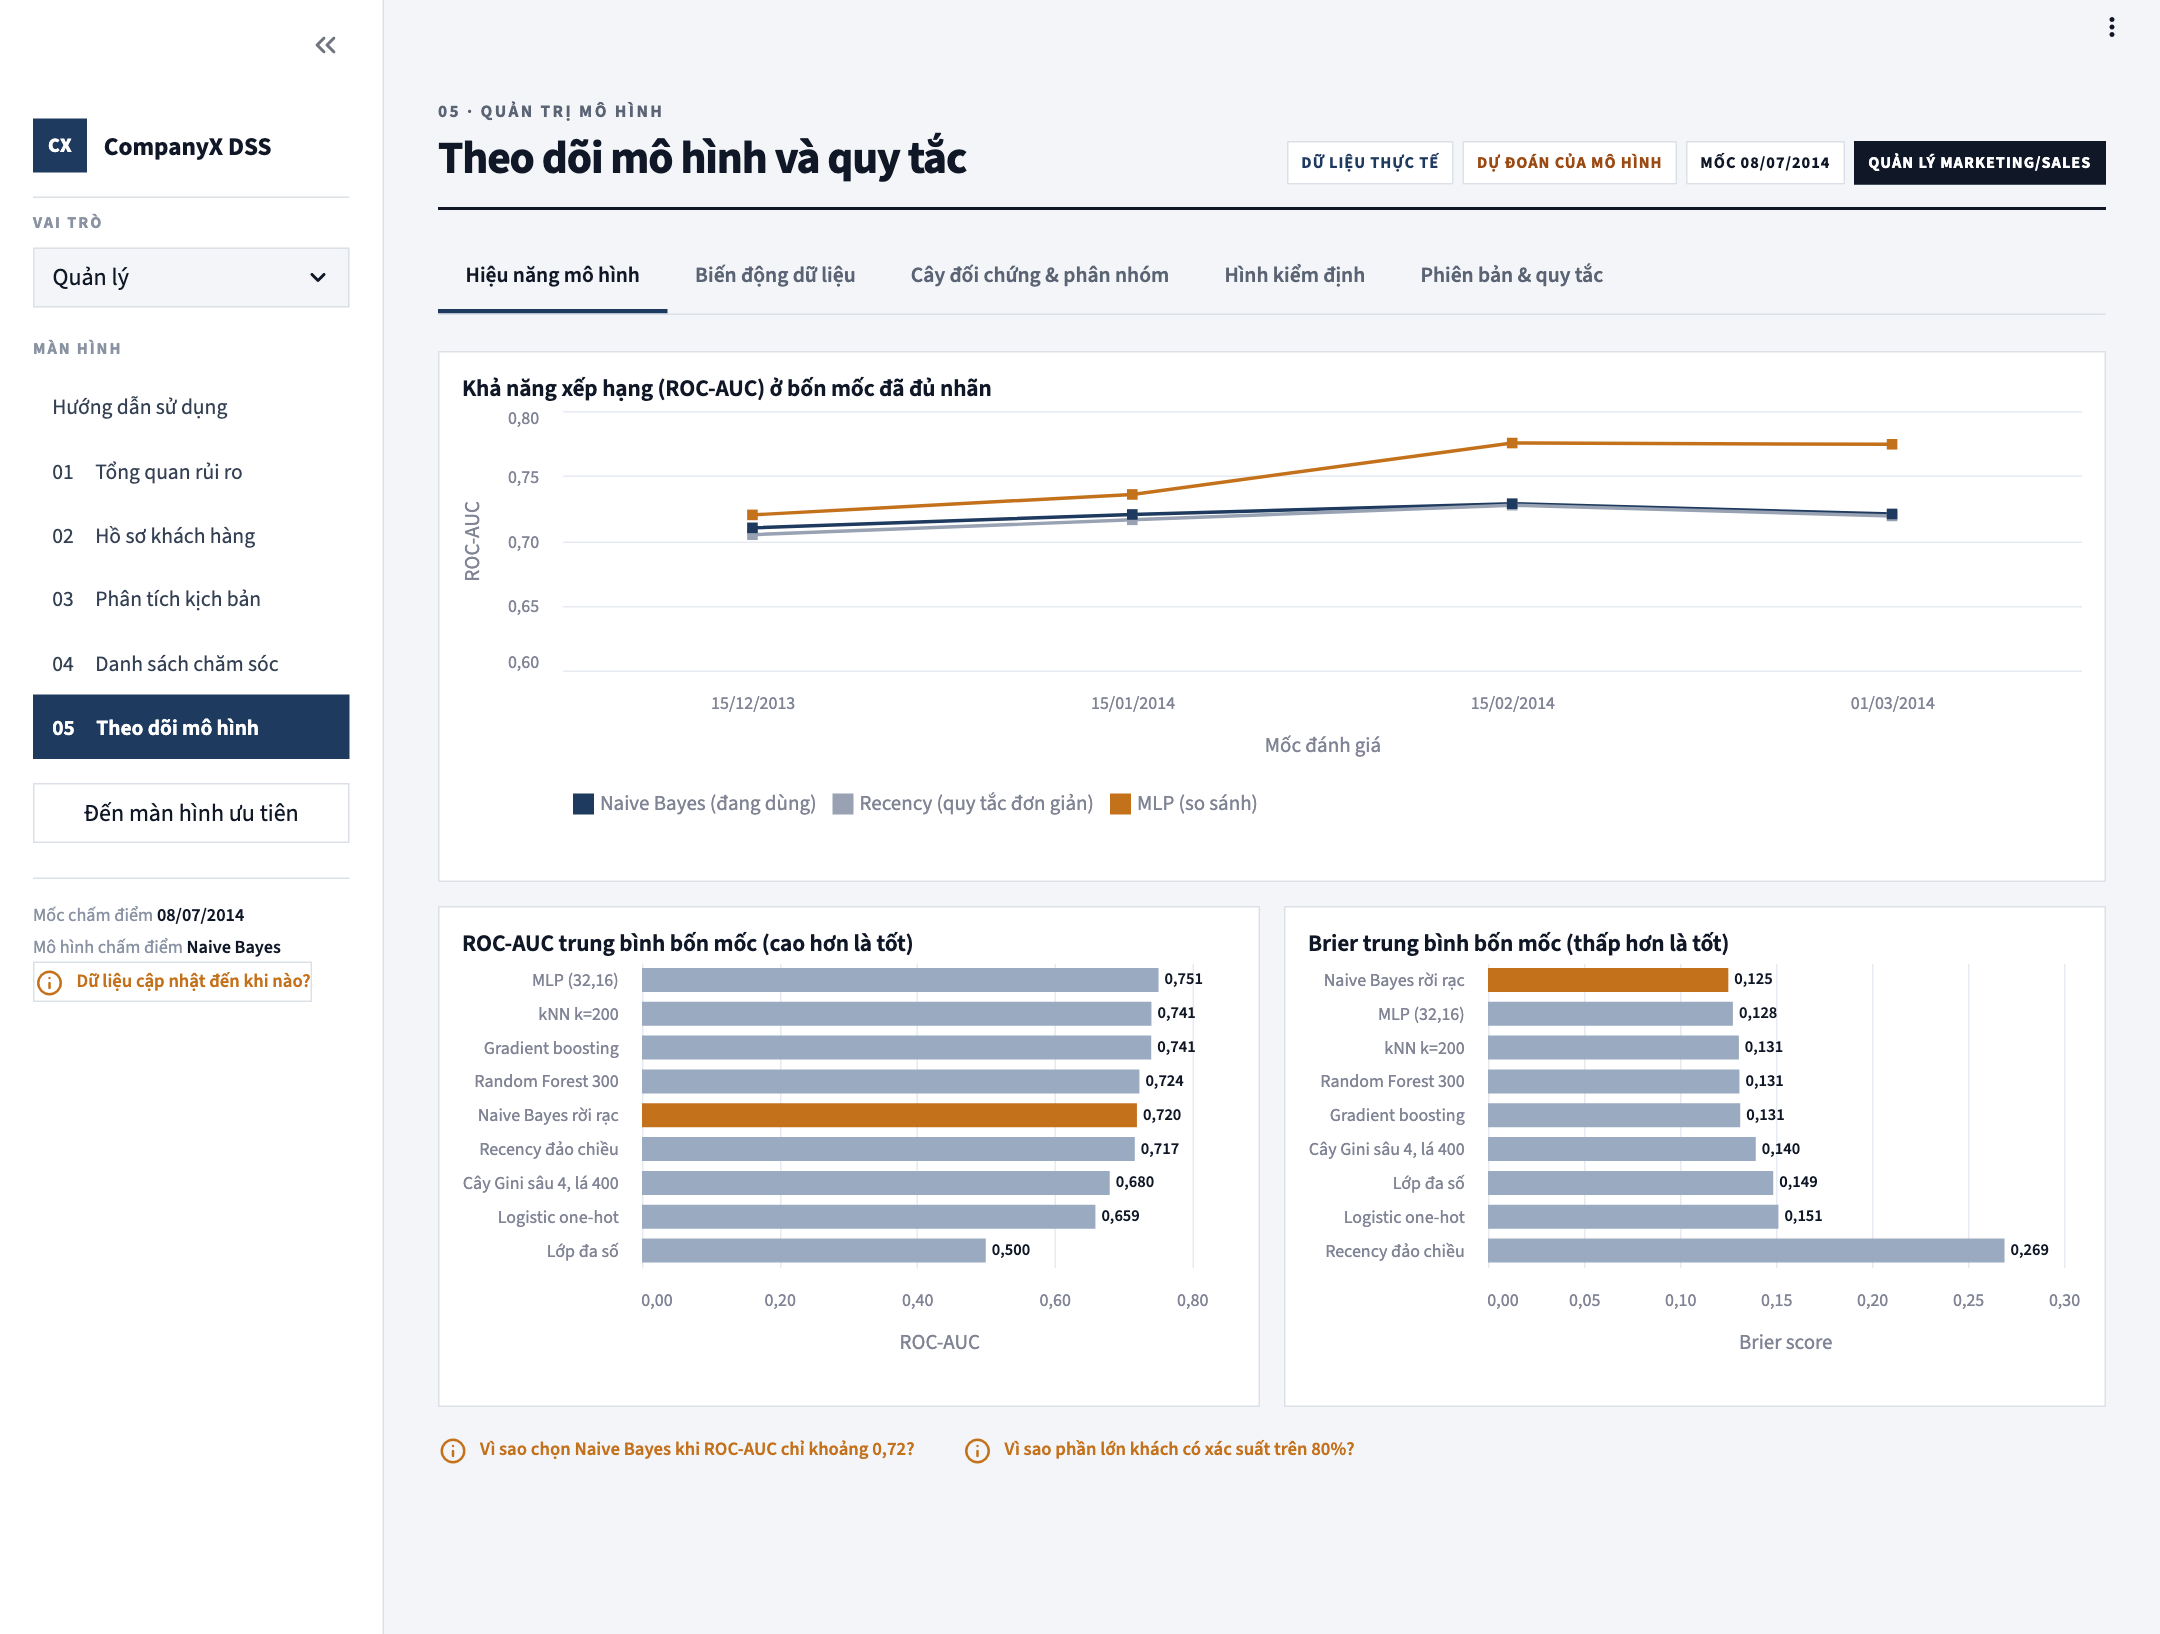
\includegraphics[width=0.95\textwidth]{d_man_hinh_5.png}
\caption{Màn hình 5: theo dõi mô hình và quy tắc, thẻ hiệu năng mô hình}
\label{fig:man5}
\end{figure}

\subsection{Hiện thực DSS: giao diện và demo}
\subsubsection{Người dùng, vai trò và màn hình}\label{sec:vaitro}
Phân hệ giao diện nhận lệnh và tham số của người dùng, chuyển cho ba phân hệ dữ liệu, mô hình và tri thức, rồi trình bày kết quả~\cite{turban2011} (Hình~\ref{fig:uims}). Giao diện là ứng dụng web Streamlit gồm năm màn hình (Bảng~\ref{tab:manhinh}) đi theo bốn pha ở Bảng~\ref{tab:quytrinh}, nhưng người dùng mở được màn hình theo thứ tự bất kỳ. Thao tác kiểu OLAP (roll-up, drill-down, slice và dice) thực hiện bằng truy vấn tổng hợp trên kho~\cite{kimball2013}, không dùng máy chủ OLAP riêng. Xác suất và tỷ lệ khách rủi ro cao không cộng dồn được (gộp hai nhóm thì phải tính lại tỷ lệ trên tổng số khách, không cộng hai tỷ lệ), nên khi gộp lên mức cao hơn hệ thống tính lại trên số khách phân biệt trong cùng một mốc. Mỗi con số trên màn hình có nhãn cho biết là dữ liệu thực tế, dự đoán của mô hình hay theo giả định, kèm ngày chấm điểm và phiên bản mô hình. Khi người quản lý thêm hoặc bớt khách, hệ thống tính lại chi phí và $Z$, kiểm tra ràng buộc ngân sách và quy tắc R2. Hình~\ref{fig:man2} minh hoạ màn hình 2 với hồ sơ khách 26339.

\begin{figure}[!htbp]
\centering
\begin{tikzpicture}[
  box/.style={draw, rounded corners=2pt, align=center, font=\small, minimum height=0.9cm},
  cert/.style={-{Stealth[length=2mm]}}]
  \node[box, text width=2.2cm, minimum height=2.2cm] (u) at (0,0) {Người dùng};
  \node[box, text width=3.0cm, minimum height=2.2cm] (m) at (5.2,0) {Phân hệ giao diện\\(quản lý hội thoại)};
  \node[box, text width=2.8cm] (d) at (10.6,1.4) {Phân hệ dữ liệu};
  \node[box, text width=2.8cm] (mo) at (10.6,0) {Phân hệ mô hình};
  \node[box, text width=2.8cm] (t) at (10.6,-1.4) {Phân hệ tri thức};
  \draw[cert] ([yshift=0.45cm]u.east) -- node[above, font=\scriptsize, text width=2.6cm, align=center] {ngôn ngữ hành động: chọn mốc, lọc, nhập tham số, duyệt} ([yshift=0.45cm]m.west);
  \draw[cert] ([yshift=-0.45cm]m.west) -- node[below, font=\scriptsize, text width=2.6cm, align=center] {ngôn ngữ hiển thị: thẻ chỉ số, biểu đồ, bảng, danh sách} ([yshift=-0.45cm]u.east);
  \draw[cert, <->, {Stealth[length=2mm]}-{Stealth[length=2mm]}] (m.east) -- (d.west);
  \draw[{Stealth[length=2mm]}-{Stealth[length=2mm]}] (m.east) -- (mo.west);
  \draw[{Stealth[length=2mm]}-{Stealth[length=2mm]}] (m.east) -- (t.west);
\end{tikzpicture}

\caption{Kiến trúc phân hệ giao diện người dùng của DSS}
\label{fig:uims}
\end{figure}

\begin{table}[!htbp]
\centering
\caption{Năm màn hình của CompanyX DSS}
\label{tab:manhinh}
\footnotesize
\begin{tabular}{p{0.6cm}p{2.8cm}p{9.2cm}p{1.8cm}}
\toprule
STT & Màn hình & Chức năng chính & Pha \\
\midrule
1 & Tổng quan rủi ro & Chọn mốc, lọc theo nhóm và hạng ABC, xem số khách, tỷ lệ khách mức Cao, phân bố xác suất, ma trận Rủi ro $\times$ Giá trị, cơ cấu năm nhóm, xu hướng kinh doanh và khách cần xem xét & Tìm hiểu \\
2 & Hồ sơ khách hàng & Tìm theo mã khách, xem RFM, lịch sử mua, \texttt{RiskScore} và \texttt{TreeScore}, luật của lá và cờ lệch giữa hai mô hình, nhóm, hạng, khuyến nghị và quy tắc đã kích hoạt & Tìm hiểu, lựa chọn \\
3 & Phân tích kịch bản & Ba thanh trượt $r$, $c$, $B$, bốn chỉ số kết quả ($Z$, số khách, chi phí, số khách giữ lại kỳ vọng), đường $Z$ theo ngân sách, lưu và so sánh kịch bản, độ nhạy, tìm mục tiêu, $Z$ theo ngân sách khi chưa biết $r$, mô phỏng, theo kênh & Thiết kế, lựa chọn \\
4 & Danh sách chăm sóc & Ngân sách và tuỳ chọn chi phí theo kênh, thêm hoặc bớt khách (bắt buộc ghi lý do), nhật ký điều chỉnh, $Z$ tích luỹ theo chi phí, bảng chi tiết giải thích vì sao khách được chọn, xuất CSV & Lựa chọn, thực hiện \\
5 & Theo dõi mô hình và quy tắc & ROC-AUC và Brier ở các mốc đã đủ nhãn so với quy tắc Recency, biến động cơ cấu khách, cây đối chứng và phân nhóm, phiên bản mô hình và quy tắc, đề xuất quy tắc mới (chờ duyệt) & Thực hiện \\
\bottomrule
\end{tabular}
\end{table}

\begin{figure}[!htbp]
\centering
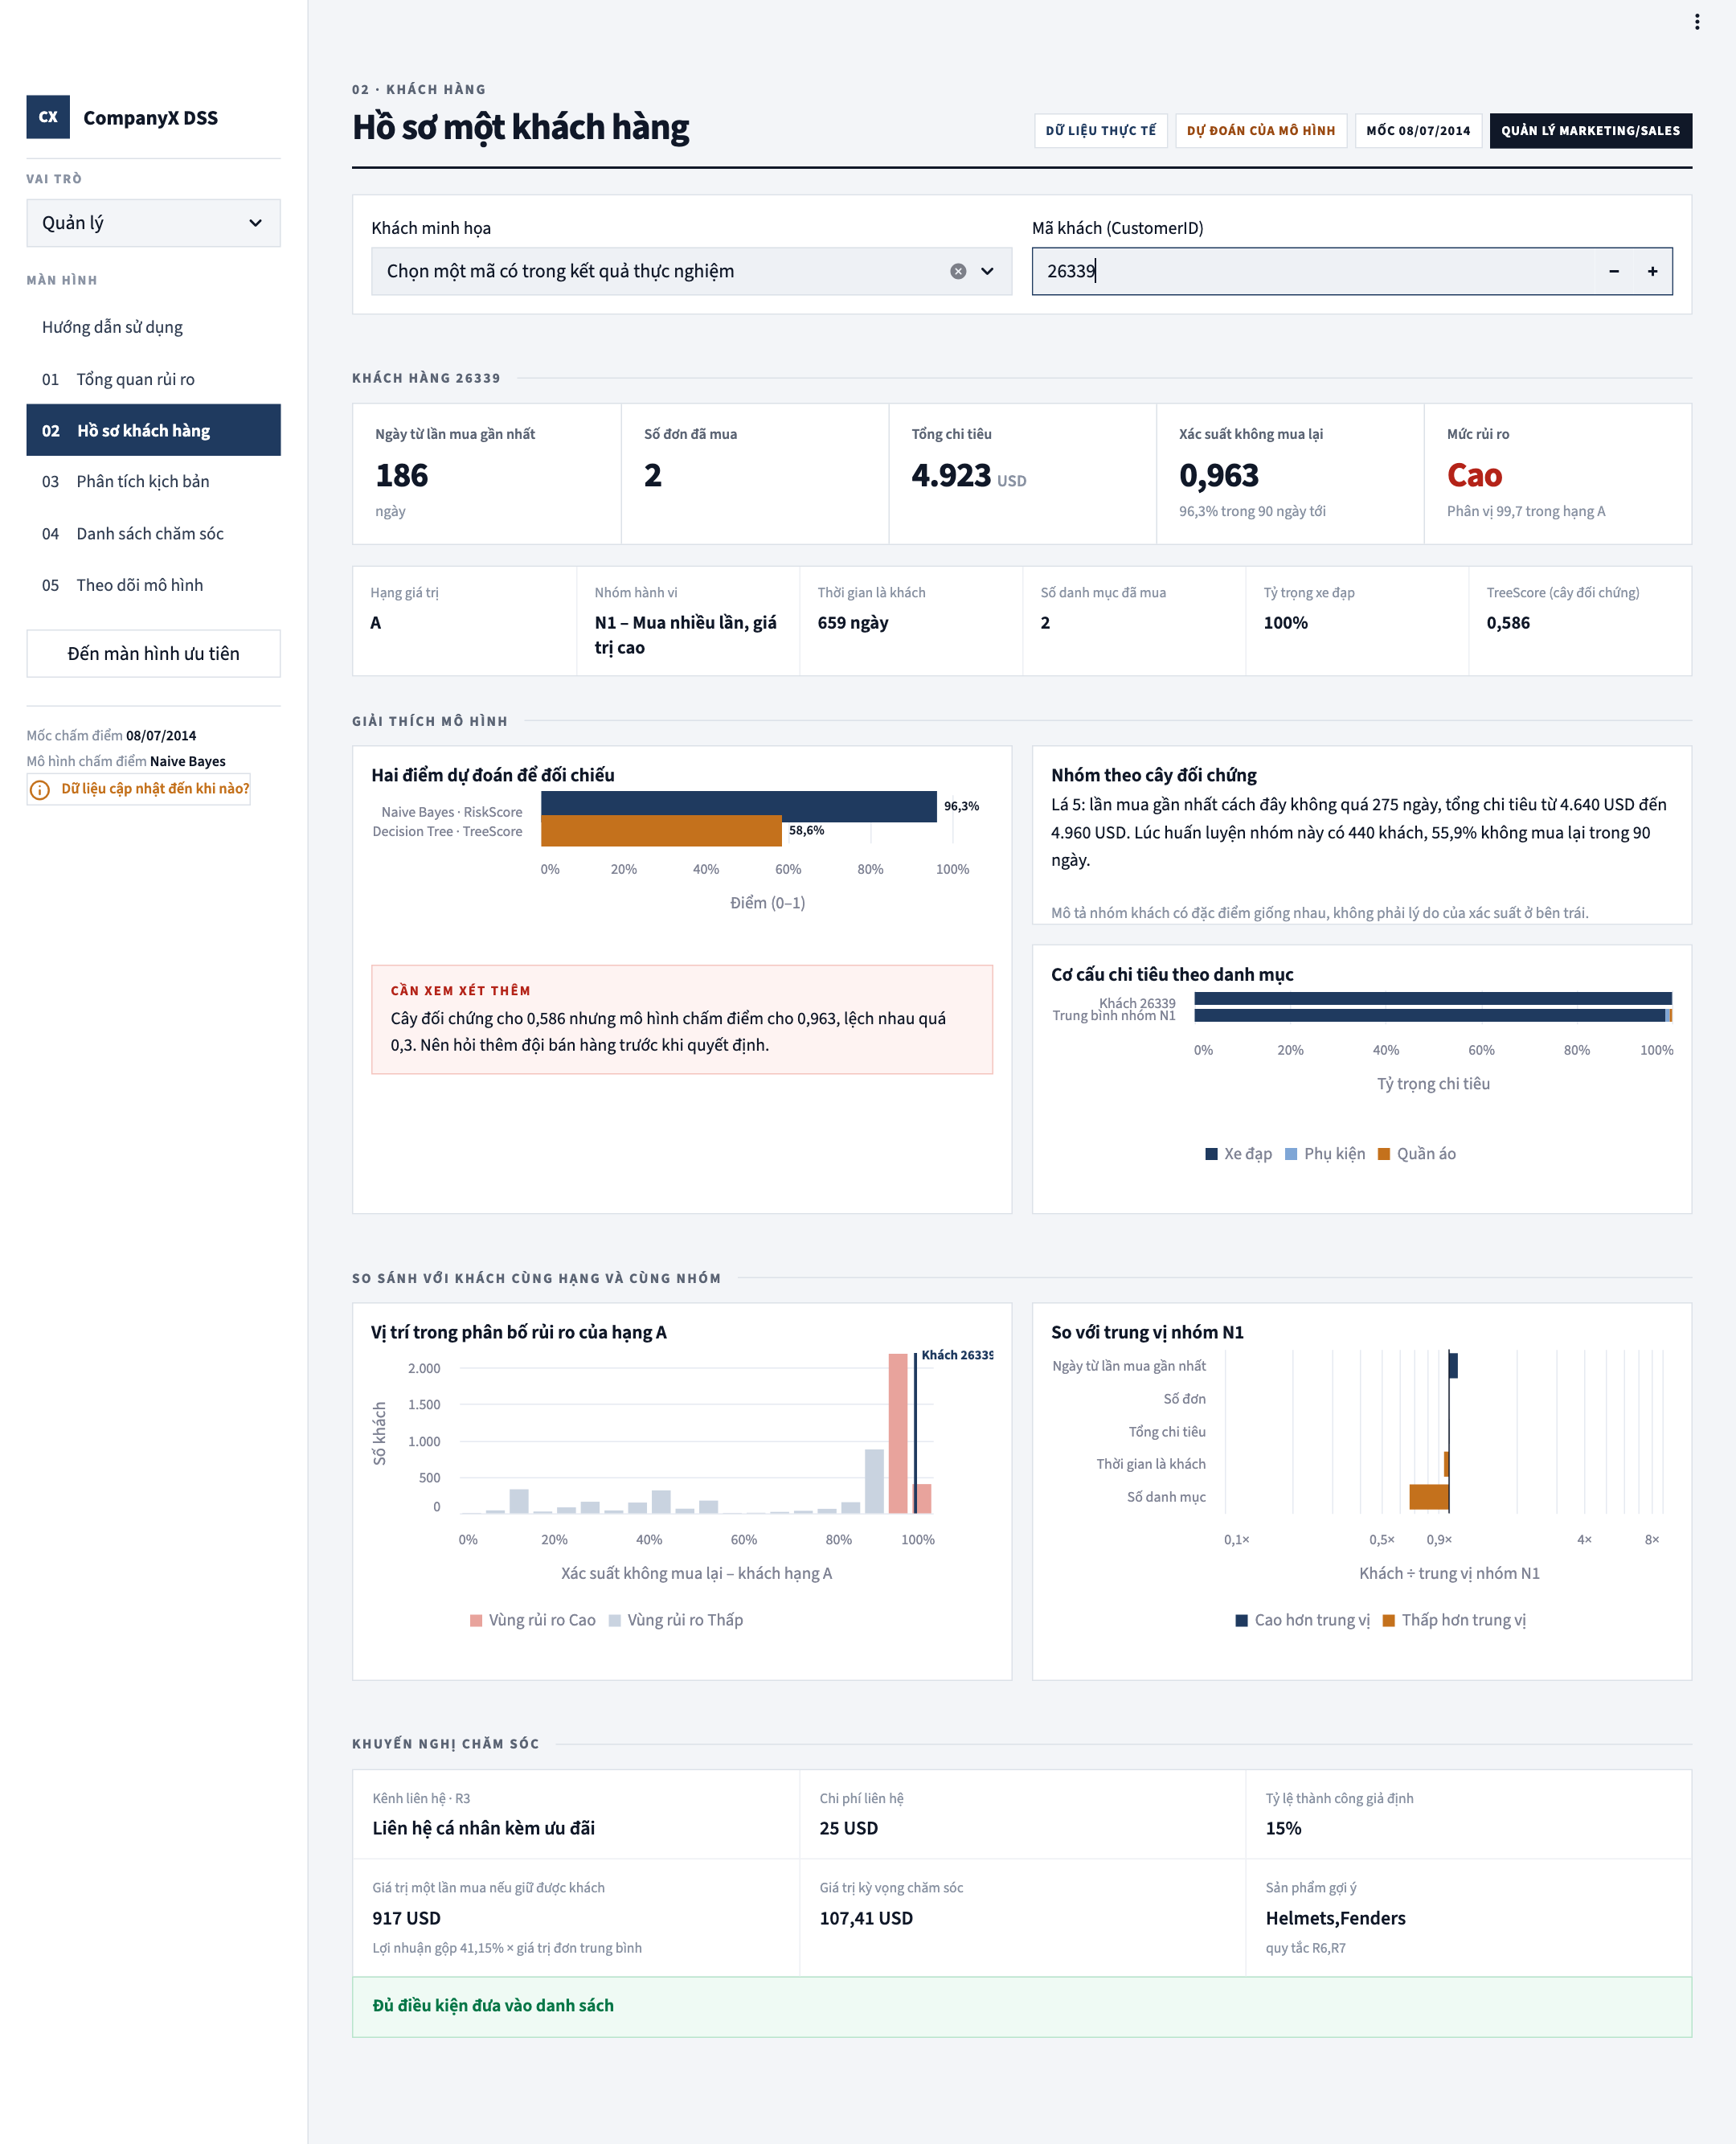
\includegraphics[width=0.95\textwidth]{d_man_hinh_2.png}
\caption{Màn hình 2: tra cứu hồ sơ và đối chiếu kết quả dự đoán của khách hàng 26339}
\label{fig:man2}
\end{figure}

Giao diện phân quyền theo ba nhóm người dùng (Bảng~\ref{tab:quyen}). Bản demo hiện thực một phần: cả ba vai trò mở được cả năm màn hình, khác nhau ở màn hình mở đầu và ở hai chức năng xuất danh sách và đề xuất quy tắc. Bản demo chưa có đăng nhập, vai trò chọn ở thanh bên chỉ để minh hoạ. Đề tài chỉ dùng giao diện đồ hoạ trên web, chưa có bộ xử lý ngôn ngữ tự nhiên như kiến trúc đầy đủ trong~\cite{turban2011}.

\begin{table}[!htbp]
\centering
\caption{Ba nhóm người dùng: quyền hạn theo thiết kế và phần đã hiện thực trong demo}
\label{tab:quyen}
\footnotesize
\begin{tabular}{p{3.0cm}p{5.4cm}p{6.0cm}}
\toprule
Người dùng & Quyền hạn theo thiết kế & Trong bản demo \\
\midrule
Quản lý Marketing/Sales & Xem, chạy kịch bản, duyệt danh sách, phê duyệt quy tắc mới hoặc sửa đổi & Mở đầu ở màn hình 1. Xuất CSV danh sách đã duyệt, đề xuất quy tắc mới (chờ duyệt) \\
Nhân viên phân tích dữ liệu & Xem, chạy chấm điểm, tạo và sửa quy tắc ở trạng thái chờ duyệt, không duyệt danh sách & Mở đầu ở màn hình 5. Chỉ xem danh sách, không có nút xuất CSV. Đề xuất quy tắc mới \\
Nhân viên chăm sóc khách hàng & Xem danh sách đã duyệt, xuất CSV, cập nhật kết quả liên hệ & Mở đầu ở màn hình 4. Xuất CSV để liên hệ khách. Không thấy mục đề xuất quy tắc \\
\bottomrule
\end{tabular}
\end{table}

\subsubsection{Công nghệ và tích hợp}\label{sec:congnghe}
Bảng~\ref{tab:congnghe} nêu các thành phần công nghệ của bản hiện thực và việc mỗi thành phần đảm nhiệm.

\begin{table}[!htbp]
\centering
\caption{Thành phần công nghệ của CompanyX DSS}
\label{tab:congnghe}
\footnotesize
\begin{tabular}{p{3.3cm}p{4.2cm}p{7.2cm}}
\toprule
Thành phần & Công nghệ & Việc đảm nhiệm \\
\midrule
Kho dữ liệu & SQL Server, CSDL \texttt{CompanyX\_DW} & Lưu các bảng của kho và các bảng \texttt{analytics} (điểm rủi ro, phân nhóm, đăng ký mô hình, quy tắc chăm sóc) \\
Mô hình và phân tích & Python, scikit-learn, scipy & Học Naive Bayes và cây, chấm điểm và sinh tệp SQL để ghi điểm vào kho, giải bài toán chọn khách bằng quy hoạch nguyên \\
Kết nối & pyodbc, ODBC Driver 18 & Nối Python với SQL Server, thông tin kết nối đọc từ biến môi trường, không ghi trong mã \\
Giao diện & Streamlit, pandas, Altair & Năm màn hình, bộ lọc, biểu đồ, xuất CSV \\
\bottomrule
\end{tabular}
\end{table}

Ứng dụng có hai chế độ đọc dữ liệu. Ở chế độ mặc định, ứng dụng đọc các tệp kết quả đã xuất (\texttt{dss\_khach.csv} và các bảng kết quả ở \texttt{results}), nên chạy được khi không có SQL Server, phù hợp cho demo. Khi đặt biến môi trường \texttt{DSS\_SOURCE=db}, ứng dụng đọc điểm rủi ro, phân vị, mức rủi ro, \texttt{TreeScore}, \texttt{TopFactors} và hạng ABC trực tiếp từ \texttt{analytics.\allowbreak CustomerRiskScore} nối với \texttt{analytics.\allowbreak CustomerSegment}, và chỉ lấy điểm của phiên bản mô hình đang dùng trong \texttt{analytics.\allowbreak ModelRegistry}. Nếu không nối được kho, ứng dụng quay về dữ liệu đã xuất và báo ở thanh bên. Các cột còn lại, như nhóm khách, kênh chăm sóc và giá trị một lần mua, vẫn đọc từ tệp đã xuất ở cả hai chế độ. Việc chọn khách theo ngân sách và các phân tích what-if được tính bằng Python trên dữ liệu đã nạp vào bộ nhớ. Điều chỉnh của người dùng và quy tắc đề xuất mới chưa được ghi ngược vào kho.

Để chạy lại hệ thống, nhóm dựng kho từ các tệp SQL (hoặc khôi phục bản sao lưu), cài môi trường Python, đặt biến môi trường kết nối, chạy chuỗi tập lệnh phân tích để sinh kết quả và các tệp SQL ghi điểm vào kho, rồi mở ứng dụng bằng lệnh \texttt{streamlit run python/app\_dss.py}.

\subsubsection{Kịch bản demo}
Bản demo dùng dữ liệu tại mốc 08/07/2014, các kết quả đã tính sẵn và lưu trong kho nên giao diện không phải chạy lại mô hình. Demo đi theo một tình huống xuyên suốt.
\begin{enumerate}
    \item Người quản lý xem tổng quan rủi ro (Hình~\ref{fig:man1}).
    \item Tra cứu khách 26339, có \texttt{RiskScore} 0,963 và \texttt{TreeScore} 0,586 (Hình~\ref{fig:man2}). Chênh lệch 0,377 vượt ngưỡng 0,3 nên DSS gắn cờ để người quản lý xem xét, không tự sửa điểm.
    \item Thử các kịch bản ngân sách (Hình~\ref{fig:man3}), xem phương án theo kênh rồi chuyển sang danh sách chăm sóc.
    \item Tại danh sách chăm sóc (Hình~\ref{fig:man4}), bớt khách 26339 kèm lý do và xuất CSV với vai trò được phép.
    \item Màn hình theo dõi (Hình~\ref{fig:man5}) cho nhân viên phân tích xem ROC-AUC, Brier, biến động dữ liệu, kết quả phân nhóm và phiên bản mô hình.
\end{enumerate}
Việc gửi chiến dịch và ghi nhận phản hồi nằm ngoài phạm vi demo, DSS cung cấp căn cứ và đề xuất, quyết định cuối thuộc về người quản lý.

\subsubsection{Các đặc điểm DSS mà hệ thống đáp ứng đầy đủ}
Trong 14 đặc điểm của DSS theo Turban và Aronson~\cite{turban2005} (Hình~\ref{fig:dac_trung_dss}), thiết kế nhắm vào ba đặc điểm gắn trực tiếp với bài toán: hỗ trợ bài toán bán cấu trúc, mô hình hoá và phân tích, và con người kiểm soát máy. Máy tính phần có cấu trúc, người quản lý quyết phần phán đoán ($r$, $c$, kênh liên hệ, duyệt danh sách, phê duyệt quy tắc), nhờ vậy bài toán bán cấu trúc giải được. Bảng~\ref{tab:dacdiem} liệt kê bốn đặc điểm mà bản triển khai đáp ứng đầy đủ, gồm ba đặc điểm trên và đặc điểm hỗ trợ nhiều phong cách ra quyết định, kèm bằng chứng trong báo cáo.

\begin{table}[!htbp]
\centering
\caption{Bốn đặc điểm DSS mà bản triển khai đáp ứng đầy đủ}
\label{tab:dacdiem}
\footnotesize
\renewcommand{\arraystretch}{1.1}
\begin{tabular}{>{\raggedright\arraybackslash}p{0.6cm}>{\raggedright\arraybackslash}p{4.6cm}>{\raggedright\arraybackslash}p{9.4cm}}
\toprule
STT & Đặc điểm & Bằng chứng \\
\midrule
1 & Giải quyết bài toán bán cấu trúc và phi cấu trúc & Hệ thống tính xác suất, $EV$ và danh sách (mục 6.2), người quản lý đặt $r$, $c$, $B$ và điều chỉnh danh sách (Hình~\ref{fig:man3}, \ref{fig:man4}) \\
6 & Hỗ trợ nhiều quy trình và phong cách ra quyết định & Lạc quan, bi quan, giá trị kỳ vọng (Bảng~\ref{tab:payoff}) và mô phỏng (Hình~\ref{fig:mophong}) \\
10 & Con người kiểm soát máy & Điều chỉnh thủ công bắt buộc có lý do, lý do ghi vào tệp xuất (Hình~\ref{fig:man4}) \\
12 & Mô hình hoá và phân tích & Phân lớp, gom cụm, luật kết hợp, quy hoạch nguyên, what-if, độ nhạy, tìm mục tiêu, mô phỏng, dự báo (Chương 5, mục 6.2 đến 6.5) \\
\bottomrule
\end{tabular}
\end{table}

\subsubsection{Đánh giá khả dụng}\label{sec:nielsen}
Khả dụng gồm ba mặt là hiệu quả, hiệu suất và mức hài lòng~\cite{iso9241}. Nhóm rà soát nội bộ giao diện theo 10 nguyên tắc của Nielsen~\cite{nielsen1994} (Bảng~\ref{tab:nielsen}, Phụ lục~\ref{sec:pl_nielsen}), gọi là nội bộ vì do chính nhóm làm, không phải chuyên gia độc lập. Nhóm tìm ra 18 vấn đề, đã sửa 14, còn 4 vấn đề nhẹ hoặc thuộc giới hạn phạm vi. Hai vấn đề cuối (số 17 và 18) được phát hiện sau đợt rà soát đầu, khi kiểm thử chức năng ở mục~\ref{sec:kiemthu}. Hai vấn đề nặng nhất (mức 3) đều đã sửa. Ứng dụng có tab Hướng dẫn sử dụng gồm năm bước và các câu hỏi thường gặp. Nhóm chưa thử với người dùng thật nên chưa kết luận về mức hài lòng.

Giới hạn còn lại của DSS: R1, R9 và nhóm đối chứng cần dữ liệu CRM, và chức năng đề xuất quy tắc mới ở màn hình 5 mới là bản trình diễn, chưa lưu vào kho. Các hạn chế này được tổng hợp ở Chương 7.

\subsubsection{Kiểm thử chức năng}\label{sec:kiemthu}
Rà soát theo Nielsen (mục~\ref{sec:nielsen}) trả lời câu hỏi giao diện có dễ dùng không. Mục này trả lời một câu hỏi khác: hệ thống có làm đúng những gì đã thiết kế ở các mục 6.1 đến 6.6.1 không. Nhóm kiểm thử hộp đen trên bản demo, tức chỉ thao tác qua giao diện rồi so kết quả hiển thị với kết quả mong đợi, không dựa vào mã nguồn.

Kết quả mong đợi lấy từ các tệp kết quả đã tính ở Chương 5 và 6 (\texttt{dss\_khach.csv} và các bảng \texttt{bang\_4\_4\_*.csv}, tương ứng Bảng~\ref{tab:abc}, \ref{tab:whatif}, \ref{tab:theokenh} và \ref{tab:payoff}), và từ truy vấn SQL trực tiếp trên kho \texttt{CompanyX\_DW}. Nhờ vậy một con số sai trên màn hình bị phát hiện ngay, thay vì chỉ nhìn bằng mắt rồi cho là đúng. Các ca được thiết kế bằng bốn kỹ thuật:
\begin{itemize}
    \item \textbf{Phân vùng tương đương:} chia đầu vào thành nhóm hợp lệ và không hợp lệ, mỗi nhóm thử một đại diện, ví dụ mã khách có điểm và mã không có trong dữ liệu.
    \item \textbf{Giá trị biên:} thử ở mức ngân sách mà danh sách đã hết khách có giá trị kỳ vọng dương ($B$ = 100.000 USD) và khi ngân sách đã dùng gần hết.
    \item \textbf{Bảng quyết định:} phân quyền theo ba vai trò ở Bảng~\ref{tab:quyen}, mỗi vai trò một ca.
    \item \textbf{Đối chiếu với kho:} con số trên giao diện phải khớp với truy vấn SQL trên các bảng analytics.
\end{itemize}
Mọi ca dùng mốc chấm điểm 08/07/2014 và phiên bản Naive Bayes đang dùng. Các ca TC01 đến TC24 chạy ở chế độ mặc định của ứng dụng (đọc tệp kết quả đã xuất), còn TC25 đối chiếu số trên màn hình với kho. Bảng~\ref{tab:kiemthu} ở Phụ lục~\ref{sec:pl_kiemthu} liệt kê đủ 25 ca theo năm màn hình, phân quyền và đối chiếu dữ liệu, kèm kết quả quan sát của từng ca.

Nhóm đã chạy đủ 25 ca. Lần chạy đầu có hai ca không khớp mong đợi. Ca TC16 thật sự thiếu chức năng nên nhóm sửa ứng dụng và chạy lại thì đạt. Ca TC23 có mong đợi viết cho thiết kế cũ (thẻ hiệu năng riêng cho mốc chấm điểm), nên nhóm đổi mong đợi theo thiết kế hiện tại, khi đó ca này đạt. Kết quả cuối: 21 ca đạt và 4 ca đạt có lưu ý (TC07, TC12, TC15 và TC19). Bốn lưu ý đều là chênh lệch nhỏ giữa mô tả và cách ứng dụng hoạt động, không ca nào cho số liệu sai.

Kiểm thử chức năng có ba giới hạn. Các ca được chạy thủ công một lần trên bản demo, chưa có bộ kiểm thử tự động để chạy lại mỗi khi sửa mã. Nhóm chưa kiểm thử hiệu năng khi nhiều người dùng truy cập cùng lúc. Nhóm cũng chưa kiểm thử bảo mật, vì bản demo chưa có đăng nhập và vai trò chỉ chọn ở thanh bên để minh hoạ.
